
%% bare_jrnl.tex
%% V1.4b
%% 2015/08/26
%% by Michael Shell
%% see http://www.michaelshell.org/
%% for current contact information.
%%
%% This is a skeleton file demonstrating the use of IEEEtran.cls
%% (requires IEEEtran.cls version 1.8b or later) with an IEEE
%% journal paper.
%%
%% Support sites:
%% http://www.michaelshell.org/tex/ieeetran/
%% http://www.ctan.org/pkg/ieeetran
%% and
%% http://www.ieee.org/

%%*************************************************************************
%% Legal Notice:
%% This code is offered as-is without any warranty either expressed or
%% implied; without even the implied warranty of MERCHANTABILITY or
%% FITNESS FOR A PARTICULAR PURPOSE! 
%% User assumes all risk.
%% In no event shall the IEEE or any contributor to this code be liable for
%% any damages or losses, including, but not limited to, incidental,
%% consequential, or any other damages, resulting from the use or misuse
%% of any information contained here.
%%
%% All comments are the opinions of their respective authors and are not
%% necessarily endorsed by the IEEE.
%%
%% This work is distributed under the LaTeX Project Public License (LPPL)
%% ( http://www.latex-project.org/ ) version 1.3, and may be freely used,
%% distributed and modified. A copy of the LPPL, version 1.3, is included
%% in the base LaTeX documentation of all distributions of LaTeX released
%% 2003/12/01 or later.
%% Retain all contribution notices and credits.
%% ** Modified files should be clearly indicated as such, including  **
%% ** renaming them and changing author support contact information. **
%%*************************************************************************


% *** Authors should verify (and, if needed, correct) their LaTeX system  ***
% *** with the testflow diagnostic prior to trusting their LaTeX platform ***
% *** with production work. The IEEE's font choices and paper sizes can   ***
% *** trigger bugs that do not appear when using other class files.       ***                          ***
% The testflow support page is at:
% http://www.michaelshell.org/tex/testflow/



\documentclass[journal]{IEEEtran}
%
% If IEEEtran.cls has not been installed into the LaTeX system files,
% manually specify the path to it like:
% \documentclass[journal]{../sty/IEEEtran}

\usepackage[spanish]{babel}
\usepackage[utf8]{inputenc}
\usepackage{url}
\usepackage{subfig}
\usepackage[pdftex]{graphicx}


% Some very useful LaTeX packages include:
% (uncomment the ones you want to load)


% *** MISC UTILITY PACKAGES ***
%
%\usepackage{ifpdf}
% Heiko Oberdiek's ifpdf.sty is very useful if you need conditional
% compilation based on whether the output is pdf or dvi.
% usage:
% \ifpdf
%   % pdf code
% \else
%   % dvi code
% \fi
% The latest version of ifpdf.sty can be obtained from:
% http://www.ctan.org/pkg/ifpdf
% Also, note that IEEEtran.cls V1.7 and later provides a builtin
% \ifCLASSINFOpdf conditional that works the same way.
% When switching from latex to pdflatex and vice-versa, the compiler may
% have to be run twice to clear warning/error messages.






% *** CITATION PACKAGES ***
%
%\usepackage{cite}
% cite.sty was written by Donald Arseneau
% V1.6 and later of IEEEtran pre-defines the format of the cite.sty package
% \cite{} output to follow that of the IEEE. Loading the cite package will
% result in citation numbers being automatically sorted and properly
% "compressed/ranged". e.g., [1], [9], [2], [7], [5], [6] without using
% cite.sty will become [1], [2], [5]--[7], [9] using cite.sty. cite.sty's
% \cite will automatically add leading space, if needed. Use cite.sty's
% noadjust option (cite.sty V3.8 and later) if you want to turn this off
% such as if a citation ever needs to be enclosed in parenthesis.
% cite.sty is already installed on most LaTeX systems. Be sure and use
% version 5.0 (2009-03-20) and later if using hyperref.sty.
% The latest version can be obtained at:
% http://www.ctan.org/pkg/cite
% The documentation is contained in the cite.sty file itself.






% *** GRAPHICS RELATED PACKAGES ***
%
\ifCLASSINFOpdf
  % \usepackage[pdftex]{graphicx}
  % declare the path(s) where your graphic files are
  % \graphicspath{{../pdf/}{../jpeg/}}
  % and their extensions so you won't have to specify these with
  % every instance of \includegraphics
  % \DeclareGraphicsExtensions{.pdf,.jpeg,.png}
\else
  % or other class option (dvipsone, dvipdf, if not using dvips). graphicx
  % will default to the driver specified in the system graphics.cfg if no
  % driver is specified.
  % \usepackage[dvips]{graphicx}
  % declare the path(s) where your graphic files are
  % \graphicspath{{../eps/}}
  % and their extensions so you won't have to specify these with
  % every instance of \includegraphics
  % \DeclareGraphicsExtensions{.eps}
\fi
% graphicx was written by David Carlisle and Sebastian Rahtz. It is
% required if you want graphics, photos, etc. graphicx.sty is already
% installed on most LaTeX systems. The latest version and documentation
% can be obtained at: 
% http://www.ctan.org/pkg/graphicx
% Another good source of documentation is "Using Imported Graphics in
% LaTeX2e" by Keith Reckdahl which can be found at:
% http://www.ctan.org/pkg/epslatex
%
% latex, and pdflatex in dvi mode, support graphics in encapsulated
% postscript (.eps) format. pdflatex in pdf mode supports graphics
% in .pdf, .jpeg, .png and .mps (metapost) formats. Users should ensure
% that all non-photo figures use a vector format (.eps, .pdf, .mps) and
% not a bitmapped formats (.jpeg, .png). The IEEE frowns on bitmapped formats
% which can result in "jaggedy"/blurry rendering of lines and letters as
% well as large increases in file sizes.
%
% You can find documentation about the pdfTeX application at:
% http://www.tug.org/applications/pdftex





% *** MATH PACKAGES ***
%
%\usepackage{amsmath}
% A popular package from the American Mathematical Society that provides
% many useful and powerful commands for dealing with mathematics.
%
% Note that the amsmath package sets \interdisplaylinepenalty to 10000
% thus preventing page breaks from occurring within multiline equations. Use:
%\interdisplaylinepenalty=2500
% after loading amsmath to restore such page breaks as IEEEtran.cls normally
% does. amsmath.sty is already installed on most LaTeX systems. The latest
% version and documentation can be obtained at:
% http://www.ctan.org/pkg/amsmath





% *** SPECIALIZED LIST PACKAGES ***
%
%\usepackage{algorithmic}
% algorithmic.sty was written by Peter Williams and Rogerio Brito.
% This package provides an algorithmic environment fo describing algorithms.
% You can use the algorithmic environment in-text or within a figure
% environment to provide for a floating algorithm. Do NOT use the algorithm
% floating environment provided by algorithm.sty (by the same authors) or
% algorithm2e.sty (by Christophe Fiorio) as the IEEE does not use dedicated
% algorithm float types and packages that provide these will not provide
% correct IEEE style captions. The latest version and documentation of
% algorithmic.sty can be obtained at:
% http://www.ctan.org/pkg/algorithms
% Also of interest may be the (relatively newer and more customizable)
% algorithmicx.sty package by Szasz Janos:
% http://www.ctan.org/pkg/algorithmicx




% *** ALIGNMENT PACKAGES ***
%
%\usepackage{array}
% Frank Mittelbach's and David Carlisle's array.sty patches and improves
% the standard LaTeX2e array and tabular environments to provide better
% appearance and additional user controls. As the default LaTeX2e table
% generation code is lacking to the point of almost being broken with
% respect to the quality of the end results, all users are strongly
% advised to use an enhanced (at the very least that provided by array.sty)
% set of table tools. array.sty is already installed on most systems. The
% latest version and documentation can be obtained at:
% http://www.ctan.org/pkg/array


% IEEEtran contains the IEEEeqnarray family of commands that can be used to
% generate multiline equations as well as matrices, tables, etc., of high
% quality.




% *** SUBFIGURE PACKAGES ***
%\ifCLASSOPTIONcompsoc
%  \usepackage[caption=false,font=normalsize,labelfont=sf,textfont=sf]{subfig}
%\else
%  \usepackage[caption=false,font=footnotesize]{subfig}
%\fi
% subfig.sty, written by Steven Douglas Cochran, is the modern replacement
% for subfigure.sty, the latter of which is no longer maintained and is
% incompatible with some LaTeX packages including fixltx2e. However,
% subfig.sty requires and automatically loads Axel Sommerfeldt's caption.sty
% which will override IEEEtran.cls' handling of captions and this will result
% in non-IEEE style figure/table captions. To prevent this problem, be sure
% and invoke subfig.sty's "caption=false" package option (available since
% subfig.sty version 1.3, 2005/06/28) as this is will preserve IEEEtran.cls
% handling of captions.
% Note that the Computer Society format requires a larger sans serif font
% than the serif footnote size font used in traditional IEEE formatting
% and thus the need to invoke different subfig.sty package options depending
% on whether compsoc mode has been enabled.
%
% The latest version and documentation of subfig.sty can be obtained at:
% http://www.ctan.org/pkg/subfig




% *** FLOAT PACKAGES ***
%
%\usepackage{fixltx2e}
% fixltx2e, the successor to the earlier fix2col.sty, was written by
% Frank Mittelbach and David Carlisle. This package corrects a few problems
% in the LaTeX2e kernel, the most notable of which is that in current
% LaTeX2e releases, the ordering of single and double column floats is not
% guaranteed to be preserved. Thus, an unpatched LaTeX2e can allow a
% single column figure to be placed prior to an earlier double column
% figure.
% Be aware that LaTeX2e kernels dated 2015 and later have fixltx2e.sty's
% corrections already built into the system in which case a warning will
% be issued if an attempt is made to load fixltx2e.sty as it is no longer
% needed.
% The latest version and documentation can be found at:
% http://www.ctan.org/pkg/fixltx2e


%\usepackage{stfloats}
% stfloats.sty was written by Sigitas Tolusis. This package gives LaTeX2e
% the ability to do double column floats at the bottom of the page as well
% as the top. (e.g., "\begin{figure*}[!b]" is not normally possible in
% LaTeX2e). It also provides a command:
%\fnbelowfloat
% to enable the placement of footnotes below bottom floats (the standard
% LaTeX2e kernel puts them above bottom floats). This is an invasive package
% which rewrites many portions of the LaTeX2e float routines. It may not work
% with other packages that modify the LaTeX2e float routines. The latest
% version and documentation can be obtained at:
% http://www.ctan.org/pkg/stfloats
% Do not use the stfloats baselinefloat ability as the IEEE does not allow
% \baselineskip to stretch. Authors submitting work to the IEEE should note
% that the IEEE rarely uses double column equations and that authors should try
% to avoid such use. Do not be tempted to use the cuted.sty or midfloat.sty
% packages (also by Sigitas Tolusis) as the IEEE does not format its papers in
% such ways.
% Do not attempt to use stfloats with fixltx2e as they are incompatible.
% Instead, use Morten Hogholm'a dblfloatfix which combines the features
% of both fixltx2e and stfloats:
%
% \usepackage{dblfloatfix}
% The latest version can be found at:
% http://www.ctan.org/pkg/dblfloatfix




%\ifCLASSOPTIONcaptionsoff
%  \usepackage[nomarkers]{endfloat}
% \let\MYoriglatexcaption\caption
% \renewcommand{\caption}[2][\relax]{\MYoriglatexcaption[#2]{#2}}
%\fi
% endfloat.sty was written by James Darrell McCauley, Jeff Goldberg and 
% Axel Sommerfeldt. This package may be useful when used in conjunction with 
% IEEEtran.cls'  captionsoff option. Some IEEE journals/societies require that
% submissions have lists of figures/tables at the end of the paper and that
% figures/tables without any captions are placed on a page by themselves at
% the end of the document. If needed, the draftcls IEEEtran class option or
% \CLASSINPUTbaselinestretch interface can be used to increase the line
% spacing as well. Be sure and use the nomarkers option of endfloat to
% prevent endfloat from "marking" where the figures would have been placed
% in the text. The two hack lines of code above are a slight modification of
% that suggested by in the endfloat docs (section 8.4.1) to ensure that
% the full captions always appear in the list of figures/tables - even if
% the user used the short optional argument of \caption[]{}.
% IEEE papers do not typically make use of \caption[]'s optional argument,
% so this should not be an issue. A similar trick can be used to disable
% captions of packages such as subfig.sty that lack options to turn off
% the subcaptions:
% For subfig.sty:
% \let\MYorigsubfloat\subfloat
% \renewcommand{\subfloat}[2][\relax]{\MYorigsubfloat[]{#2}}
% However, the above trick will not work if both optional arguments of
% the \subfloat command are used. Furthermore, there needs to be a
% description of each subfigure *somewhere* and endfloat does not add
% subfigure captions to its list of figures. Thus, the best approach is to
% avoid the use of subfigure captions (many IEEE journals avoid them anyway)
% and instead reference/explain all the subfigures within the main caption.
% The latest version of endfloat.sty and its documentation can obtained at:
% http://www.ctan.org/pkg/endfloat
%
% The IEEEtran \ifCLASSOPTIONcaptionsoff conditional can also be used
% later in the document, say, to conditionally put the References on a 
% page by themselves.




% *** PDF, URL AND HYPERLINK PACKAGES ***
%
%\usepackage{url}
% url.sty was written by Donald Arseneau. It provides better support for
% handling and breaking URLs. url.sty is already installed on most LaTeX
% systems. The latest version and documentation can be obtained at:
% http://www.ctan.org/pkg/url
% Basically, \url{my_url_here}.




% *** Do not adjust lengths that control margins, column widths, etc. ***
% *** Do not use packages that alter fonts (such as pslatex).         ***
% There should be no need to do such things with IEEEtran.cls V1.6 and later.
% (Unless specifically asked to do so by the journal or conference you plan
% to submit to, of course. )


% correct bad hyphenation here
\hyphenation{op-tical net-works semi-conduc-tor}


\begin{document}
	
\renewcommand{\tablename}{Tabla} 
	
	
%
% paper title
% Titles are generally capitalized except for words such as a, an, and, as,
% at, but, by, for, in, nor, of, on, or, the, to and up, which are usually
% not capitalized unless they are the first or last word of the title.
% Linebreaks \\ can be used within to get better formatting as desired.
% Do not put math or special symbols in the title.
\title{Sistema de Monitoreo de Signos Vitales\\ Utilizando IoT}
%
%
% author names and IEEE memberships
% note positions of commas and nonbreaking spaces ( ~ ) LaTeX will not break
% a structure at a ~ so this keeps an author's name from being broken across
% two lines.
% use \thanks{} to gain access to the first footnote area
% a separate \thanks must be used for each paragraph as LaTeX2e's \thanks
% was not built to handle multiple paragraphs
%

\author{María Elsi Bernabé Aparicio, Carlos Alberto Granados Puerto,\\ Nayeli Vega García, Rubén Ortega González\\
Escuela Superior de Cómputo I.P.N. México D.F.\\
Tel. 57-29-6000 ext. 52000 y 52021. E-mail: elsibill@gmail.com, c.granados.puerto@gmail.com}% <-this % stops a space
%\thanks{M. Shell was with the Department
%of Electrical and Computer Engineering, Georgia Institute of Technology, Atlanta,
%GA, 30332 USA e-mail: (see http://www.michaelshell.org/contact.html).}% <-this % stops a space
%\thanks{J. Doe and J. Doe are with Anonymous University.}% <-this % stops a space
%\thanks{Manuscript received April 19, 2005; revised August 26, 2015.}}

% note the % following the last \IEEEmembership and also \thanks - 
% these prevent an unwanted space from occurring between the last author name
% and the end of the author line. i.e., if you had this:
% 
% \author{....lastname \thanks{...} \thanks{...} }
%                     ^------------^------------^----Do not want these spaces!
%
% a space would be appended to the last name and could cause every name on that
% line to be shifted left slightly. This is one of those "LaTeX things". For
% instance, "\textbf{A} \textbf{B}" will typeset as "A B" not "AB". To get
% "AB" then you have to do: "\textbf{A}\textbf{B}"
% \thanks is no different in this regard, so shield the last } of each \thanks
% that ends a line with a % and do not let a space in before the next \thanks.
% Spaces after \IEEEmembership other than the last one are OK (and needed) as
% you are supposed to have spaces between the names. For what it is worth,
% this is a minor point as most people would not even notice if the said evil
% space somehow managed to creep in.



% The paper headers
%\markboth{Journal of \LaTeX\ Class Files,~Vol.~14, No.~8, August~2015}%
%{Shell \MakeLowercase{\textit{et al.}}: Bare Demo of IEEEtran.cls for IEEE Journals}
% The only time the second header will appear is for the odd numbered pages
% after the title page when using the twoside option.
% 
% *** Note that you probably will NOT want to include the author's ***
% *** name in the headers of peer review papers.                   ***
% You can use \ifCLASSOPTIONpeerreview for conditional compilation here if
% you desire.




% If you want to put a publisher's ID mark on the page you can do it like
% this:
%\IEEEpubid{0000--0000/00\$00.00~\copyright~2015 IEEE}
% Remember, if you use this you must call \IEEEpubidadjcol in the second
% column for its text to clear the IEEEpubid mark.



% use for special paper notices
%\IEEEspecialpapernotice{(Invited Paper)}




% make the title area
\maketitle

% As a general rule, do not put math, special symbols or citations
% in the abstract or keywords.
\begin{abstract}
En este trabajo terminal se plantea el desarrollo del prototipo de un sistema embebido que permite el monitoreo remoto de la frecuencia cardíaca y temperatura corporal de una persona. El cálculo de la frecuencia cardíaca se realiza basado en técnicas de procesamiento digital de señales, logrando el cálculo de ésta con una eficiencia superior al 98\%.
\end{abstract}

% Note that keywords are not normally used for peerreview papers.
\renewcommand{\IEEEkeywordsname}{Palabras clave}
\begin{IEEEkeywords}
Frecuencia cardíaca, procesamiento digital de señales, sistema embebido.
\end{IEEEkeywords}



% For peer review papers, you can put extra information on the cover
% page as needed:
% \ifCLASSOPTIONpeerreview
% \begin{center} \bfseries EDICS Category: 3-BBND \end{center}
% \fi
%
% For peerreview papers, this IEEEtran command inserts a page break and
% creates the second title. It will be ignored for other modes.
\IEEEpeerreviewmaketitle



\section{Introducción}
% The very first letter is a 2 line initial drop letter followed
% by the rest of the first word in caps.
% 
% form to use if the first word consists of a single letter:
% \IEEEPARstart{A}{demo} file is ....
% 
% form to use if you need the single drop letter followed by
% normal text (unknown if ever used by the IEEE):
% \IEEEPARstart{A}{}demo file is ....
% 
% Some journals put the first two words in caps:
% \IEEEPARstart{T}{his demo} file is ....
% 
% Here we have the typical use of a "T" for an initial drop letter
% and "HIS" in caps to complete the first word.
%\IEEEPARstart{T}{his} demo file is intended to serve as a ``starter file''
%for IEEE journal papers produced under \LaTeX\ using
%IEEEtran.cls version 1.8b and later.
% You must have at least 2 lines in the paragraph with the drop letter
% (should never be an issue)
Los signos vitales son mediciones de las funciones más básicas del cuerpo, es decir, indicadores que reflejan el estado físico del paciente y sus órganos vitales, cuyas variaciones expresan cambios ocurridos en el organismo, algunos de índole fisiológico y otros de tipo patológico \cite{aguayoChile} \cite{cobo2011}. Los cuatros signos vitales principales que se examinan de forma rutinaria son: frecuencia cardíaca, frecuencia respiratoria, presión arterial y temperatura corporal. \\

En este trabajo se desarrolló un sistema embebido para el cálculo de la frecuencia cardíaca y la obtención de la temperatura corporal. \\

Los valores del pulso arterial se miden a partir de la frecuencia cardíaca, es decir, el número de pulsaciones o latidos del corazón que ocurren en un minuto. Cuando el corazón bombea sangre a través de las arterias, éstas se expanden y contraen con el flujo sanguíneo. La frecuencia cardíaca común para personas sanas mayores a 10 años varía de 60 a 100 latidos por minuto, sin embargo, la frecuencia cardíaca varía dependiendo de diferentes factores, como: la edad, el sexo, la actividad física, la temperatura, entre otros. \cite{valoresFreq} \\

La temperatura corporal representa el estado térmico del organismo y expresa el balance entre la producción y pérdida de calor en el cuerpo \cite{cobo2011}. Ya que la temperatura depende de la parte del cuerpo en donde se realice la medición, ya sea interna o externa, por lo que se considera un rango de $36^{\circ}C$ a $37^{\circ}C$ para la temperatura \textit{normal} del cuerpo humano. Además la temperatura corporal de una persona sana varía a lo largo del día dependiendo del sexo, la actividad reciente, el consumo de alimentos y líquidos, la hora del día y, en el caso de las mujeres, la etapa del ciclo menstrual \cite{signosvitales2016}. \\

De acuerdo con la Organización para la Cooperación y el Desarrollo Económicos (OCDE), México tiene 2.2 médicos practicantes y 2.6 enfermeras practicantes por cada 1,000 habitantes, mucho menos que los promedios de la OCDE de 3.3 y 9.1 respectivamente. El número de camas hospitalarias también es considerablemente bajo, con 1.6 camas por cada 1,000 habitantes, comparado con 4.8 camas por cada 1,000 de la OCDE; siendo de los promedios más bajos dentro de los países que conforman la OCDE \cite{ocde2016}. Aunado a esto, existe una gran demanda de atención médica y con los pocos espacios disponibles el servicio ofrecido se vuelve lento e ineficiente. \\

En consecuencia, existe una necesidad creciente de utilizar la tecnología para monitorear, informar y analizar de manera remota los signos vitales del paciente sin la necesidad de acudir con el personal médico. Esta forma de monitoreo beneficia tanto al paciente como a los hospitales pues se podrán tener registros de las mediciones de los signos en cualquier momento sin interrumpir la vida cotidiana del paciente y se tendrá la seguridad de que en una emergencia se podrá contactar a los familiares del paciente o a un médico para tratar la condición a tiempo.

\section{Metodología}

Para la realización de este trabajo terminal se decidió utilizar la metodología descrita por el Modelo en V ya que ofrece una visión detallada de los diversos pasos e interacciones relacionados con el proceso de desarrollo y puede considerarse como un flujo de trabajo comúnmente utilizado \cite{perez2006V}. \\

\begin{figure}[htbp!]
	\centering
	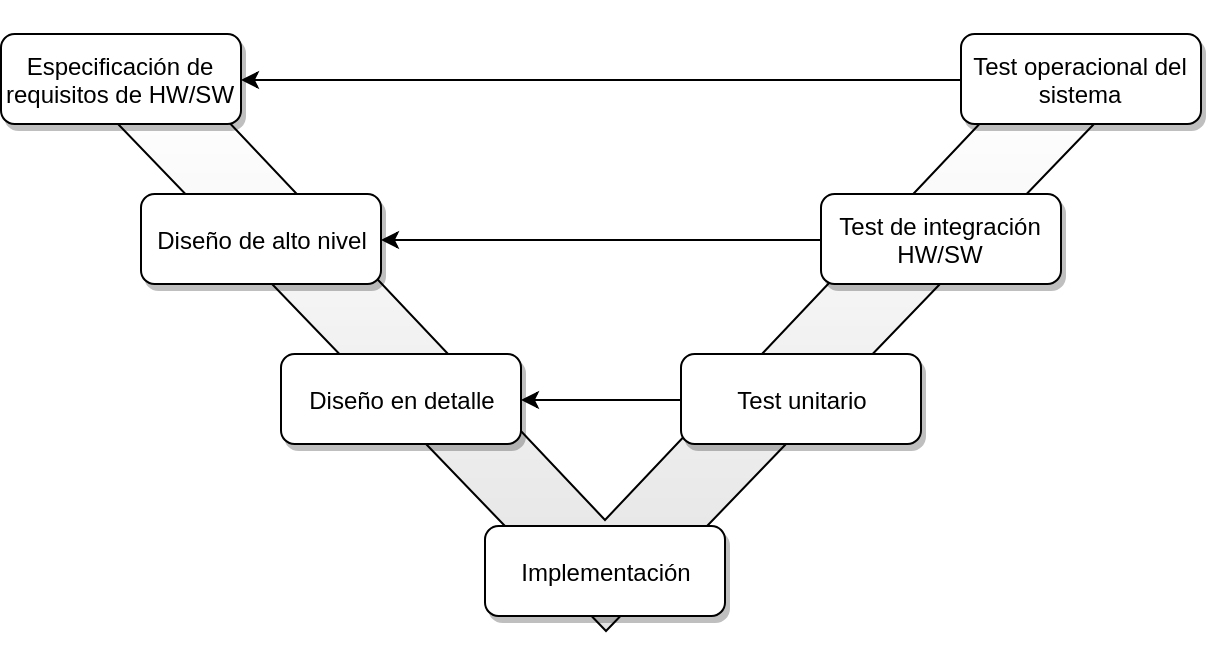
\includegraphics[width=2.5in]{imagenes/metodologiaV.png}
	\caption{Fases del Modelo en V.}
	\label{fig:IntroduccionMetodologia}
\end{figure}

Siguiendo este modelo se pretende definir y documentar los diferentes requerimientos del sistema a implementar, seguido de un diseño global que permitirá obtener una visión general del sistema identificando las funciones que deberá cumplir y asignarlas a los diferentes componentes, ya sea de hardware o software, para posteriormente detallar este diseño e implementar cada uno de los módulos. \\

A cada fase del diseño corresponde una fase de pruebas con las que, después de la implementación del diseño, se verifica y valida que los resultados obtenidos cumplen con los requerimientos establecidos para el sistema.

%\subsection{Sistemas embebidos}
%Un sistema embebido es una combinación de hardware y software integrado para realizar una función particular \cite{vahid1999}.
%
%\subsection{Internet de las cosas (IoT)}
%El Internet de las cosas (IoT) es un concepto que describe una red de dispositivos interconectados que tiene capacidades avanzadas para interactuar con dispositivos y también con seres humanos y el mundo físico circundante para realizar una variedad de tareas \cite{vermesanIoT}.\\
%
%En este contexto, el uso de sensores en dispositivos IoT proveen una conexión entre estos y el mundo físico, por ejemplo, el acelerómetro, giroscopio, micrófono, sensor de luz, entre muchos otros, que permiten aplicaciones más eficientes y fáciles de usar \cite{laneIoT}. \\
%
%En general, la arquitectura de los dispositivos IoT comprende cuatro componentes principales: detección, red, procesamiento de datos y capa de aplicación \cite{arquitecturaIoT}.

% needed in second column of first page if using \IEEEpubid
%\IEEEpubidadjcol

\subsection{Arquitectura física del sistema}
En la figura \ref{fig:DisenoArquiFisica} se muestra la arquitectura física del sistema, la cual abarca el diseño de la aplicación móvil así como el sistema embebido encargado de realizar las mediciones y el procesamiento de los datos.\\

La arquitectura se divide en dos módulos:
\begin{enumerate}
	\item Aplicación Móvil: se refiere a la aplicación móvil que proporciona un punto de acceso al usuario para la consulta de las mediciones realizadas por los sensores y procesadas por el microcontrolador en el sistema embebido. El usuario recibe el mensaje de texto en su dispositivo móvil y la aplicación móvil obtiene los datos de dicho mensaje mediante el número telefónico registrado en la información del paciente. 
	
	\item Sistema Embebido: abarca todos los componentes que integran el sistema embebido como tal. Para este prototipo se utilizó una tarjeta que facilita las conexiones con el microcontrolador \textit{dsPIC30F4013}, en donde se conecta el sensor analógico tipo fotopletismógrafo \textit{Pulse Sensor} para obtener la señal de pulso cardíaco del paciente a través de una entrada analógica, este señal es digitalizada en el ADC del microcontrolador para procesarla y obtener la frecuencia cardíaca. Para la obtención de la temperatura, se empleó el sensor digital \textit{MAX30205} con una resolución de $0.00390625^{\circ}C$. Estos valores se envían al módulo de comunicación, con el que se realizará la comunicación con la red 3G/4G utilizando el \textit{módulo 4G con el chip LARA R-202} y con el dispositivo móvil.
\end{enumerate}

\begin{figure}[htbp!]
	\centering
	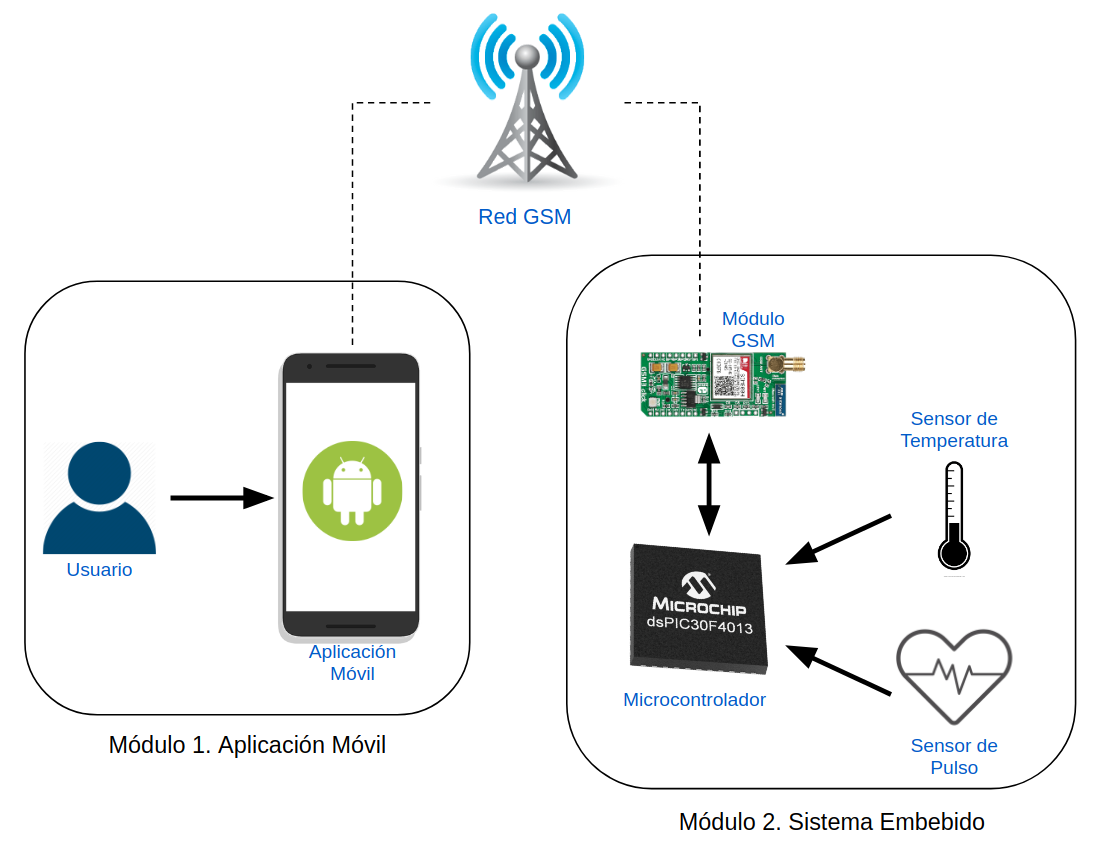
\includegraphics[width=2.5in]{imagenes/arquifisica.png}
	\caption{Arquitectura física del sistema}
	\label{fig:DisenoArquiFisica}
\end{figure}

\subsection{Obtención de la frecuencia cardíaca}
Para obtener la señal de pulso cardíaco, se configuró el periférico AN2 del microcontrolador para ser la entrada del convertidor analógico-digital de 12 bits incluido en el microcontrolador. Se definió la frecuencia de muestreo mediante el teorema de Nyquist ($Fs \geq 2f$). Considerando una frecuencia cardíaca de $210\ lpm$, se tiene que $Fs \geq 7.3332\ Hz$, pero se redondeó a $8\ Hz$ para trabajar con un valor entero. Por lo tanto frecuencias mayores a partir de $8\ Hz$ serían adecuadas para obtener la información necesaria para el tratamiento de la señal digital.\\

En la figura \ref{fig:conexionPS} se muestra la conexión del sensor de pulso con la tarjeta y su uso sobre el dedo índice.

\begin{figure}[htbp!]
	\centering
	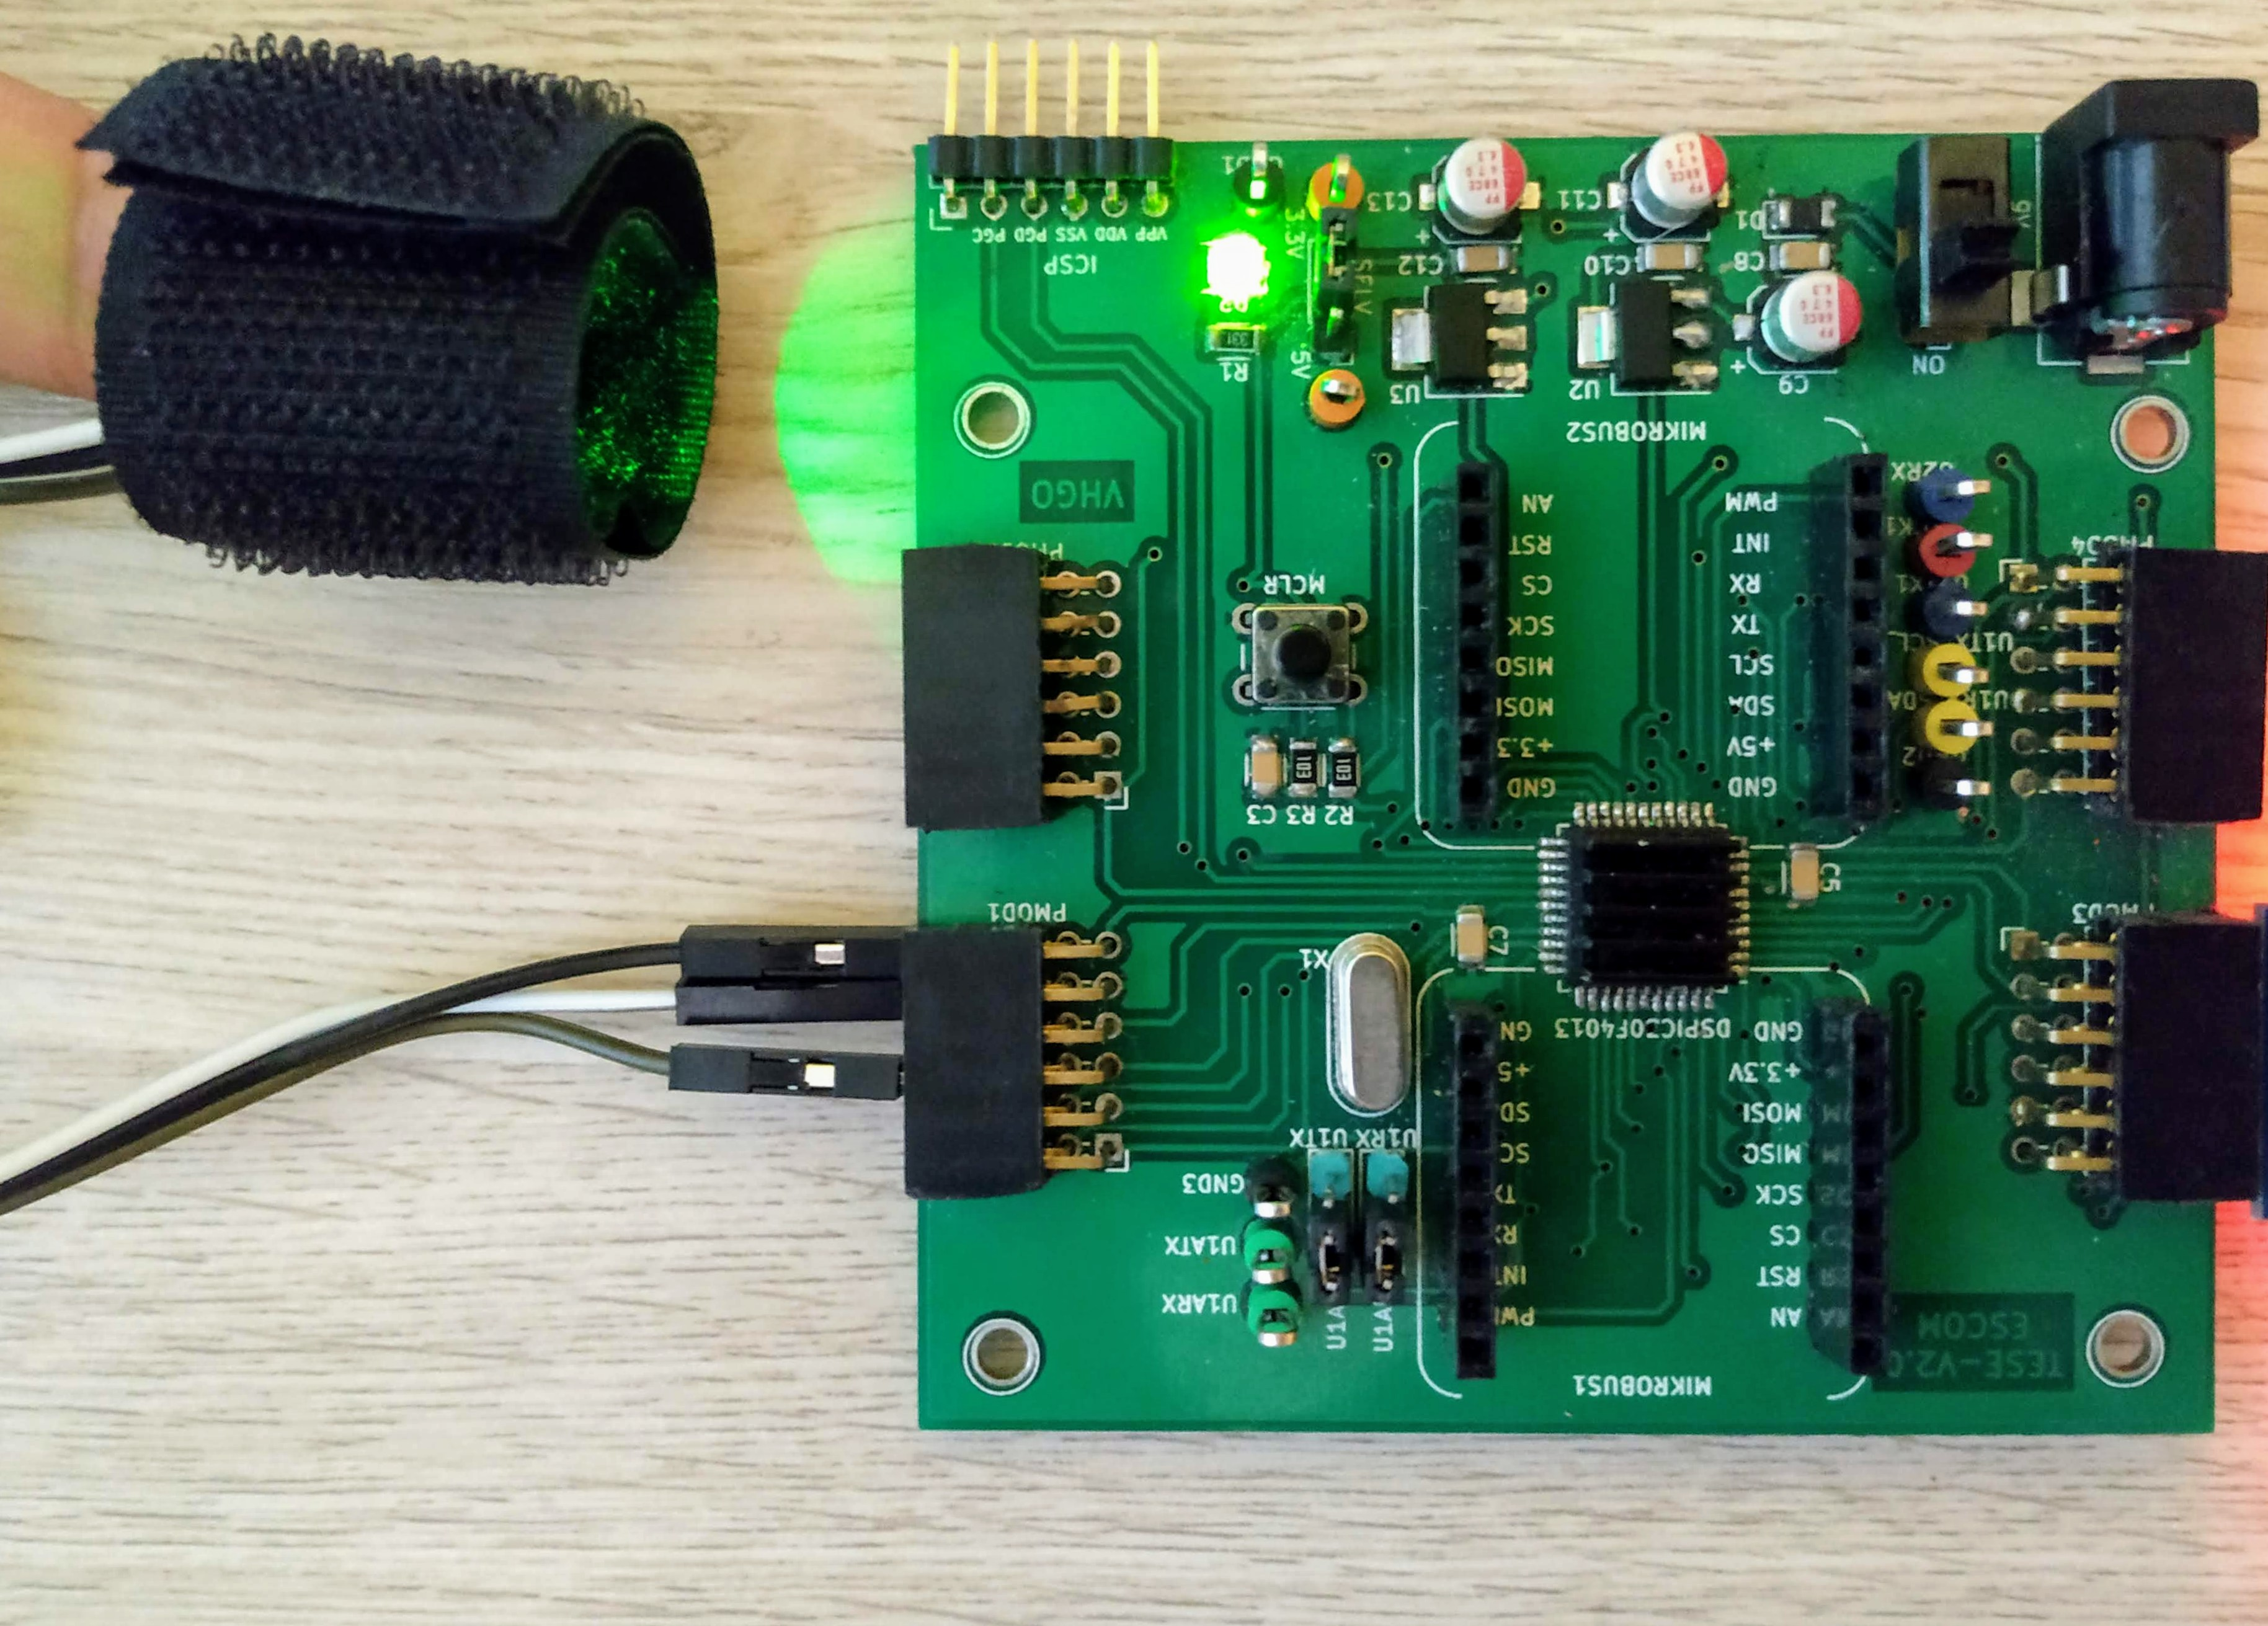
\includegraphics[width=2.5in]{AvancesPruebas/imagenes/conexionPS.jpg}
	\caption{Conexión de Pulse Sensor con el microcontrolador.}
	\label{fig:conexionPS}
\end{figure}

Para el cálculo de la frecuencia cardíaca se utilizó la ecuación dada por:
\begin{equation}
	\label{eq:lpm}
	lpm = \frac{Fs}{pos} * 60
\end{equation}

donde:
\begin{itemize}
	\item $lpm$: frecuencia cardíaca expresada en latidos por minuto.
	\item $Fs$: frecuencia de muestreo.
	\item $pos$: índice de la posición del segundo valor máximo de la autocorrelación.\\
\end{itemize}

Dado que la fórmula (\ref{eq:lpm}) depende de la frecuencia de muestreo ($Fs$) y la posición del valor máximo de la autocorrelación ($pos$), se realizaron pruebas variando esta frecuencia desde $8\ Hz$ hasta $512\ Hz$. \\

En la tabla \ref{sensorPulso:resultadosCalculoFs} se muestra un resumen de los resultados obtenidos al aplicar la fórmula (\ref{eq:lpm}) a las frecuencias mencionadas con el fin de obtener los resultados posibles de la frecuencia cardíaca expresada en latidos por minuto. 

\begin{table}[htbp!]
	\begin{center}
		\begin{tabular}{|l|l|l|l|l|l|l|}
			\hline
			\textbf{pos / Fs} & \textbf{8 Hz} & \textbf{16 Hz} & \textbf{...} & \textbf{128 Hz} & \textbf{...} & \textbf{512 Hz} \\
			\hline \hline
			\textbf{3} & 160 & 320 & ... & 2560 & ... & 10240 \\
			\hline
			\textbf{4} & 120 & 240 & ... & 1920 & ... & 7680 \\
			\hline
			\textbf{5} & 96 & 192 & ... & 1536 & ... & 6144 \\
			\hline
			\textbf{...} & ... & ... & ... & ... & ... & ...  \\
			\hline
			\textbf{83} & 5.783 & 11.566 & ... & 92.530 & ... & 370.120 \\
			\hline
			\textbf{84} & 5.714 & 11.429 & ... & 91.429 & ... & 365.714 \\
			\hline
			\textbf{85} & 5.647 & 11.294 & ... & 90.353 & ... & 361.412 \\
			\hline
			\textbf{86} & 5.581 & 11.163 & ... & 89.302 & ... & 357.209 \\
			\hline
			\textbf{87} & 5.517 & 11.034 & ... & 88.276 & ... & 353.103 \\
			\hline
			\textbf{...} & ... & ... & ... & ... & ... & ...  \\
			\hline
			\textbf{148} & 3.243 & 6.486 & ... & 51.892 & ... & 207.568 \\
			\hline
			\textbf{149} & 3.221 & 6.443 & ... & 51.544 & ... & 206.174 \\
			\hline
			\textbf{150} & 3.2 & 6.4 & ... & 51.2 & ... & 204.8 \\
			\hline
		\end{tabular}
		\caption{Cálculo de frecuencia cardíaca.}
		\label{sensorPulso:resultadosCalculoFs}
	\end{center}
\end{table}

De los resultados mostrados en la tabla  \ref{sensorPulso:resultadosCalculoFs}, se observó que a menor $Fs$, más amplio es el rango de valores faltantes, por ejemplo, a $8\ Hz$ no se encuentran valores entre los $120$ y $96\ lpm$, lo que sucede con todas las frecuencias consideradas en ciertos valores, sin embargo, se determinó que para la frecuencia de $128\ Hz$ se tenía un rango de valores continuos hasta los $94\ lpm$ y con un rango de error de $0.84\%$ hasta $120\ lpm$, permitiendo tener una aproximación de los valores esperados sin sobrepasar la memoria de datos del microcontrolador de 2 KB. \\

Para realizar el cálculo de la frecuencia cardíaca se implementó un algoritmo para obtener la autocorrelación de la señal. La ecuación está dada por:

\begin{equation}
	\label{eq:autocorr}
	Cxx[n] = \frac{1}{N} \sum_{m=0}^{N-1-n}x[m]x[m+n]
\end{equation}

donde: 
\begin{itemize}
	\item $Cxx$: valor de la autocorrelación para un punto un particular.
	\item $n$: índice del arreglo de autocorrelación.
	\item $m$: índice del arreglo de la señal digital.
	\item $N$: cantidad de muestras para la autocorrelación.\\
\end{itemize}

Para definir la cantidad de muestras ($N$) necesarias para obtener el resultado de la autocorrelación, se realizaron 80 pruebas en las que se digitalizaron $4096$ valores utilizando el ADC del microcontrolador y se procesaron con un programa en C, en el que se aplicaba el algoritmo de autocorrelación considerando $16$ muestras y hasta $4096$, aumentando $16$ muestras para cada cálculo. Con esto se determinó el error porcentual de los resultados comparados con las mediciones reales de la frecuencia cardíaca obtenida con el método de palpación. \\

De esos resultados se observó que la cantidad de muestras influía en el resultado del cálculo de la frecuencia cardíaca y que la cantidad de muestras con un menor error ($1.17\%$) fue de $1600$. \\

El algoritmo de autocorrelación se implementó en el microcontrolador utilizando dos arreglos de 150 valores de tal manera que en uno se almacenaran los valores del ADC y en otro los valores resultantes de la autocorrelación para cada $n$, como se indica en la fórmula (\ref{eq:autocorr}). De esta manera se realiza el cálculo al vuelo, es decir, no se requiere esperar a obtener las $1600$ muestras para comenzar el cálculo de la autocorrelación y obtener cada valor $Cxx$, sino que se calculan parcialmente todos los valores para $Cxx$ conforme se termina la digitalización de la señal en el ADC hasta completar las $1600$ muestras. \\

Antes de comenzar con el cálculo de la autocorrelación se aplica un offset de $-2048$ a los valores obtenidos del ADC, ya que éste nos entrega valores entre $0$ y $4095$. Al aplicar el offset se realiza un desplazamiento de la señal para centrarlo en el eje $x$ como se muestra en la figura \ref{fig:offset}. \\

\begin{figure}[htbp!]
	\centering
	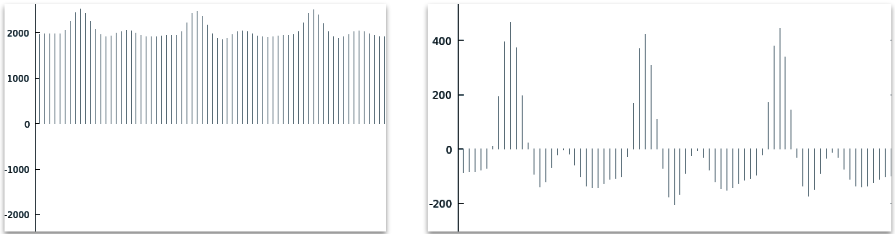
\includegraphics[width=3.2in]{AvancesPruebas/imagenes/offset.png}
	\caption{Señal digital antes y después de aplicar el offset.}
	\label{fig:offset}
\end{figure}

Posteriormente se realiza el ventaneo de la señal digital aplicando la ventana de Hamming con un tamaño de $1600$ muestras. La ventana de Hamming está dada por la siguiente fórmula: 

\begin{equation}
	\label{eq_hamming}
	w(n) = 0.54 - 0.46 * cos(\frac{2\pi n}{N})
\end{equation}

Debido a que el cálculo de los $1600$ valores de la ventana, incrementa considerablemente el tiempo de procesamiento para cada muestra, se decidió almacenar los valores de la ventana en la memoria de programa del microcontrolador con el formato Q15, reduciendo así el tiempo de ejecución y evitando que se omitan valores dentro del tiempo de muestreo. \\

En la figura \ref{fig:ventaneo} se observa el resultado del ventaneo de la señal. \\

\begin{figure}[htbp!]
	\centering
	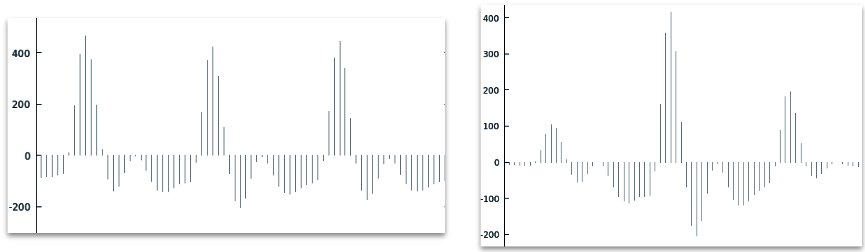
\includegraphics[width=3.2in]{AvancesPruebas/imagenes/ventaneo.png}
	\caption{Señal digital antes y después de realizar el ventaneo.}
	\label{fig:ventaneo}
\end{figure}

Al término del cálculo de los valores de la autocorrelación, se realizó la búsqueda del segundo valor máximo (omitiendo el valor máximo ubicado en la posición $0$ del arreglo $Cxx$ ya que este corresponde con la energía de la señal, y la diferencia del máximo inicial al segundo máximo representa frecuencia fundamental de la señal) para obtener la posición de este valor y así poder calcular la frecuencia cardíaca con la fórmula (\ref{eq:lpm}).

En la figura \ref{fig:autocorr} se muestra el resultado de la autocorrelación y el valor máximo de interés del que se busca su posición. \\

\begin{figure}[htbp!]
	\centering
	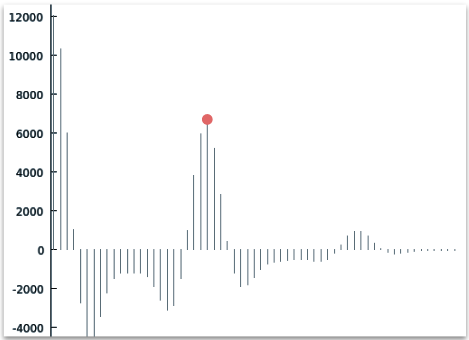
\includegraphics[width=2.3in]{AvancesPruebas/imagenes/autocorr.png}
	\caption{Resultado de la autocorrelación de la señal digital de pulso cardíaco.}
	\label{fig:autocorr}
\end{figure}

\subsection{Obtención de la temperatura}
Para obtener la medición de temperatura corporal del sensor de temperatura MAX30205, se configuró la interfaz I2C del microcontrolador a una frecuencia de trabajo de $400\ KHz$. En la figura \ref{fig:DiagramaMAX30205} se muestra el diagrama de tiempo que describe el procedimiento que debe ser seguido para establecer la comunicación entre ambos componentes.\\

\begin{figure}[htbp!]
	\centering
	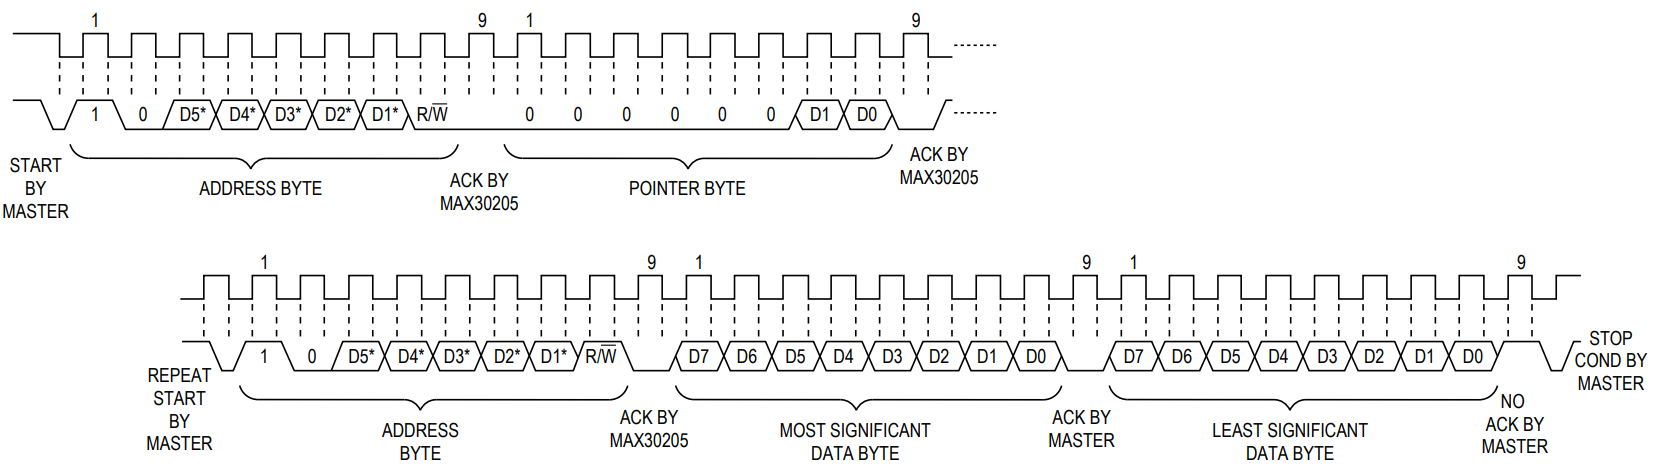
\includegraphics[width=3.5in]{AvancesPruebas/imagenes/diagramaI2C.png}
	\caption{Diagrama de tiempo I2C del sensor MAX30205.}
	\label{fig:DiagramaMAX30205}
\end{figure}

La conexión entre el sensor de temperatura y el microcontrolador se realizó mediante las terminales SDA y SCL configuradas como salida respectivamente. En la figura \ref{fig:ConexionFisicaMAX30205} se muestra la conexión física mediante el MikroBUS.

\begin{figure}[htbp!]
	\centering
	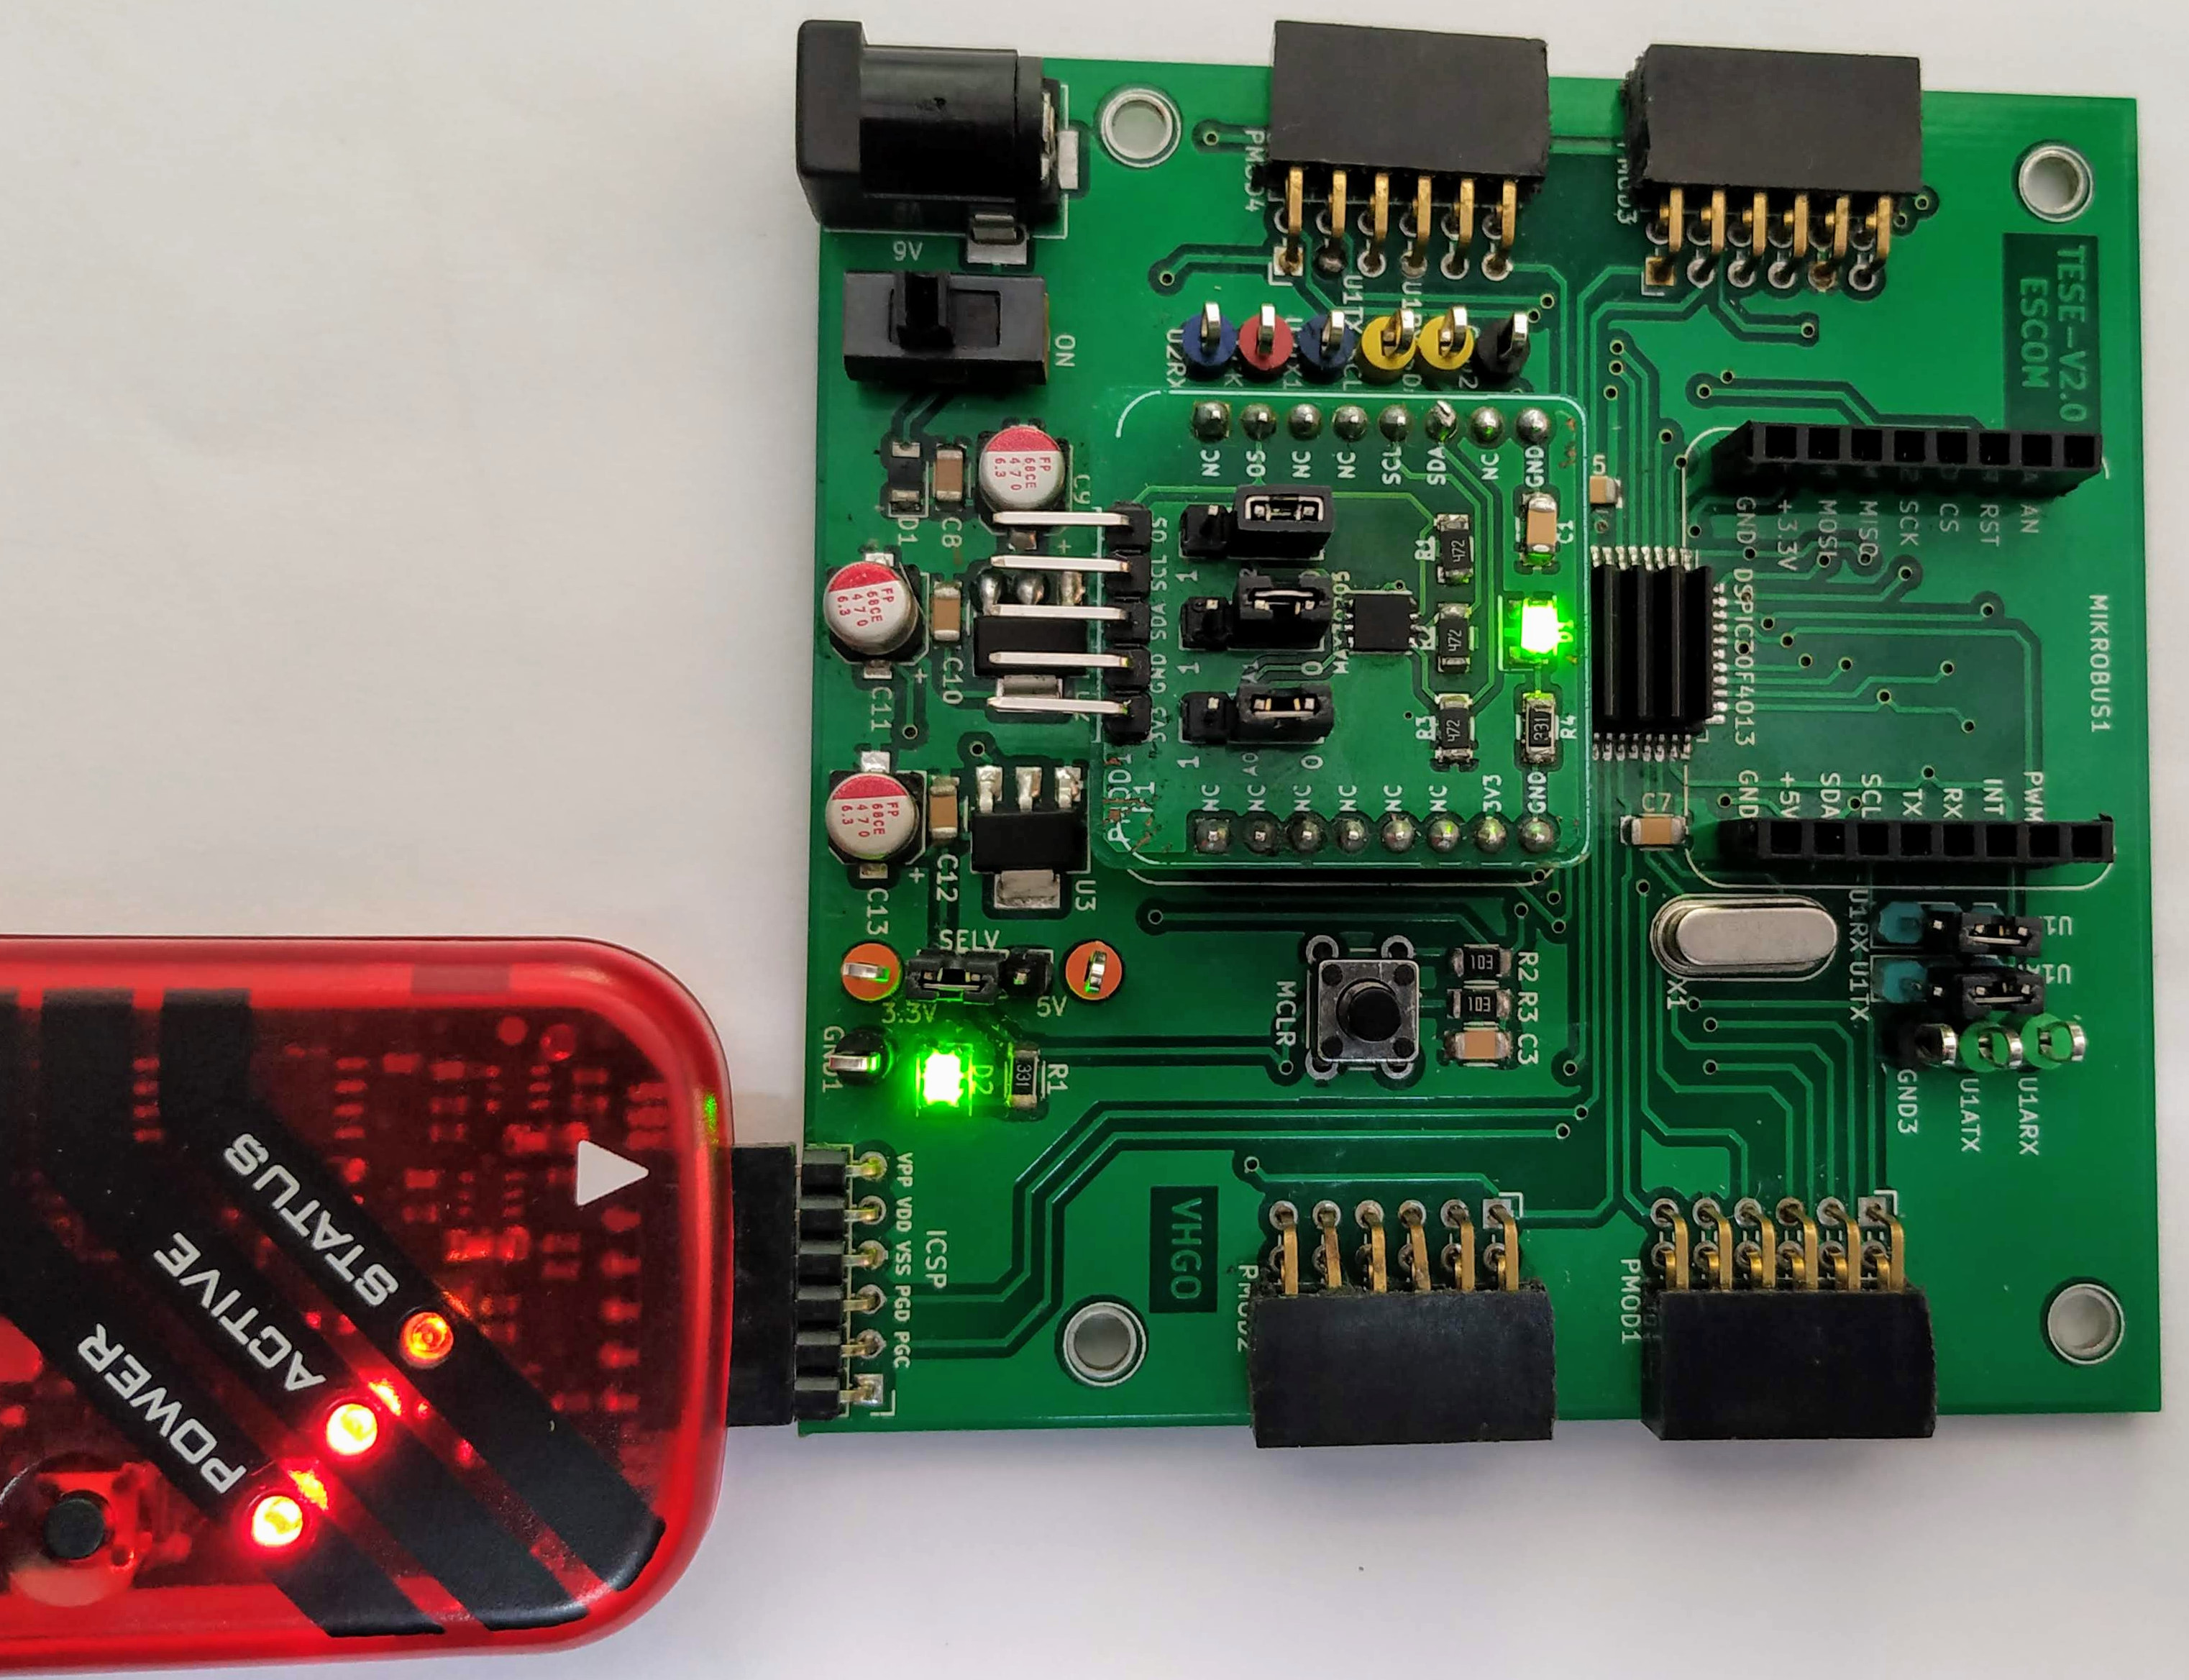
\includegraphics[width=2.5in]{AvancesPruebas/imagenes/MAX30205ConexionFisica.jpg}
	\caption{Conexión física del sensor MAX30205.}
	\label{fig:ConexionFisicaMAX30205}
\end{figure}

El sensor entrega los valores de temperatura en dos partes de 8 bits cada una. Para obtener el valor real de la medición se utilizó la siguiente fórmula:

\begin{equation}
	temp = MSB + (0.00390625 * LSB)
\end{equation}

donde: 
\begin{itemize}
	\item $temp$: valor de la temperatura corporal.
	\item $MSB$: primer byte enviado por el sensor, la parte entera del valor.
	\item $LSB$: segundo byte enviado por el sensor, la parte decimal del valor.
\end{itemize}


\subsection{Envío del mensaje de texto}
La comunicación con el módulo de comunicación se estableció configurando el UART2 del microcontrolador a una taza de transferencia de $19200\ baudios$ y mediante comandos AT se envía un mensaje de texto a un número telefónico específico. La conexión física se muestra en las figura \ref{fig:ConexionFisicaGSM}.

\begin{figure}[htbp!]
	\centering
	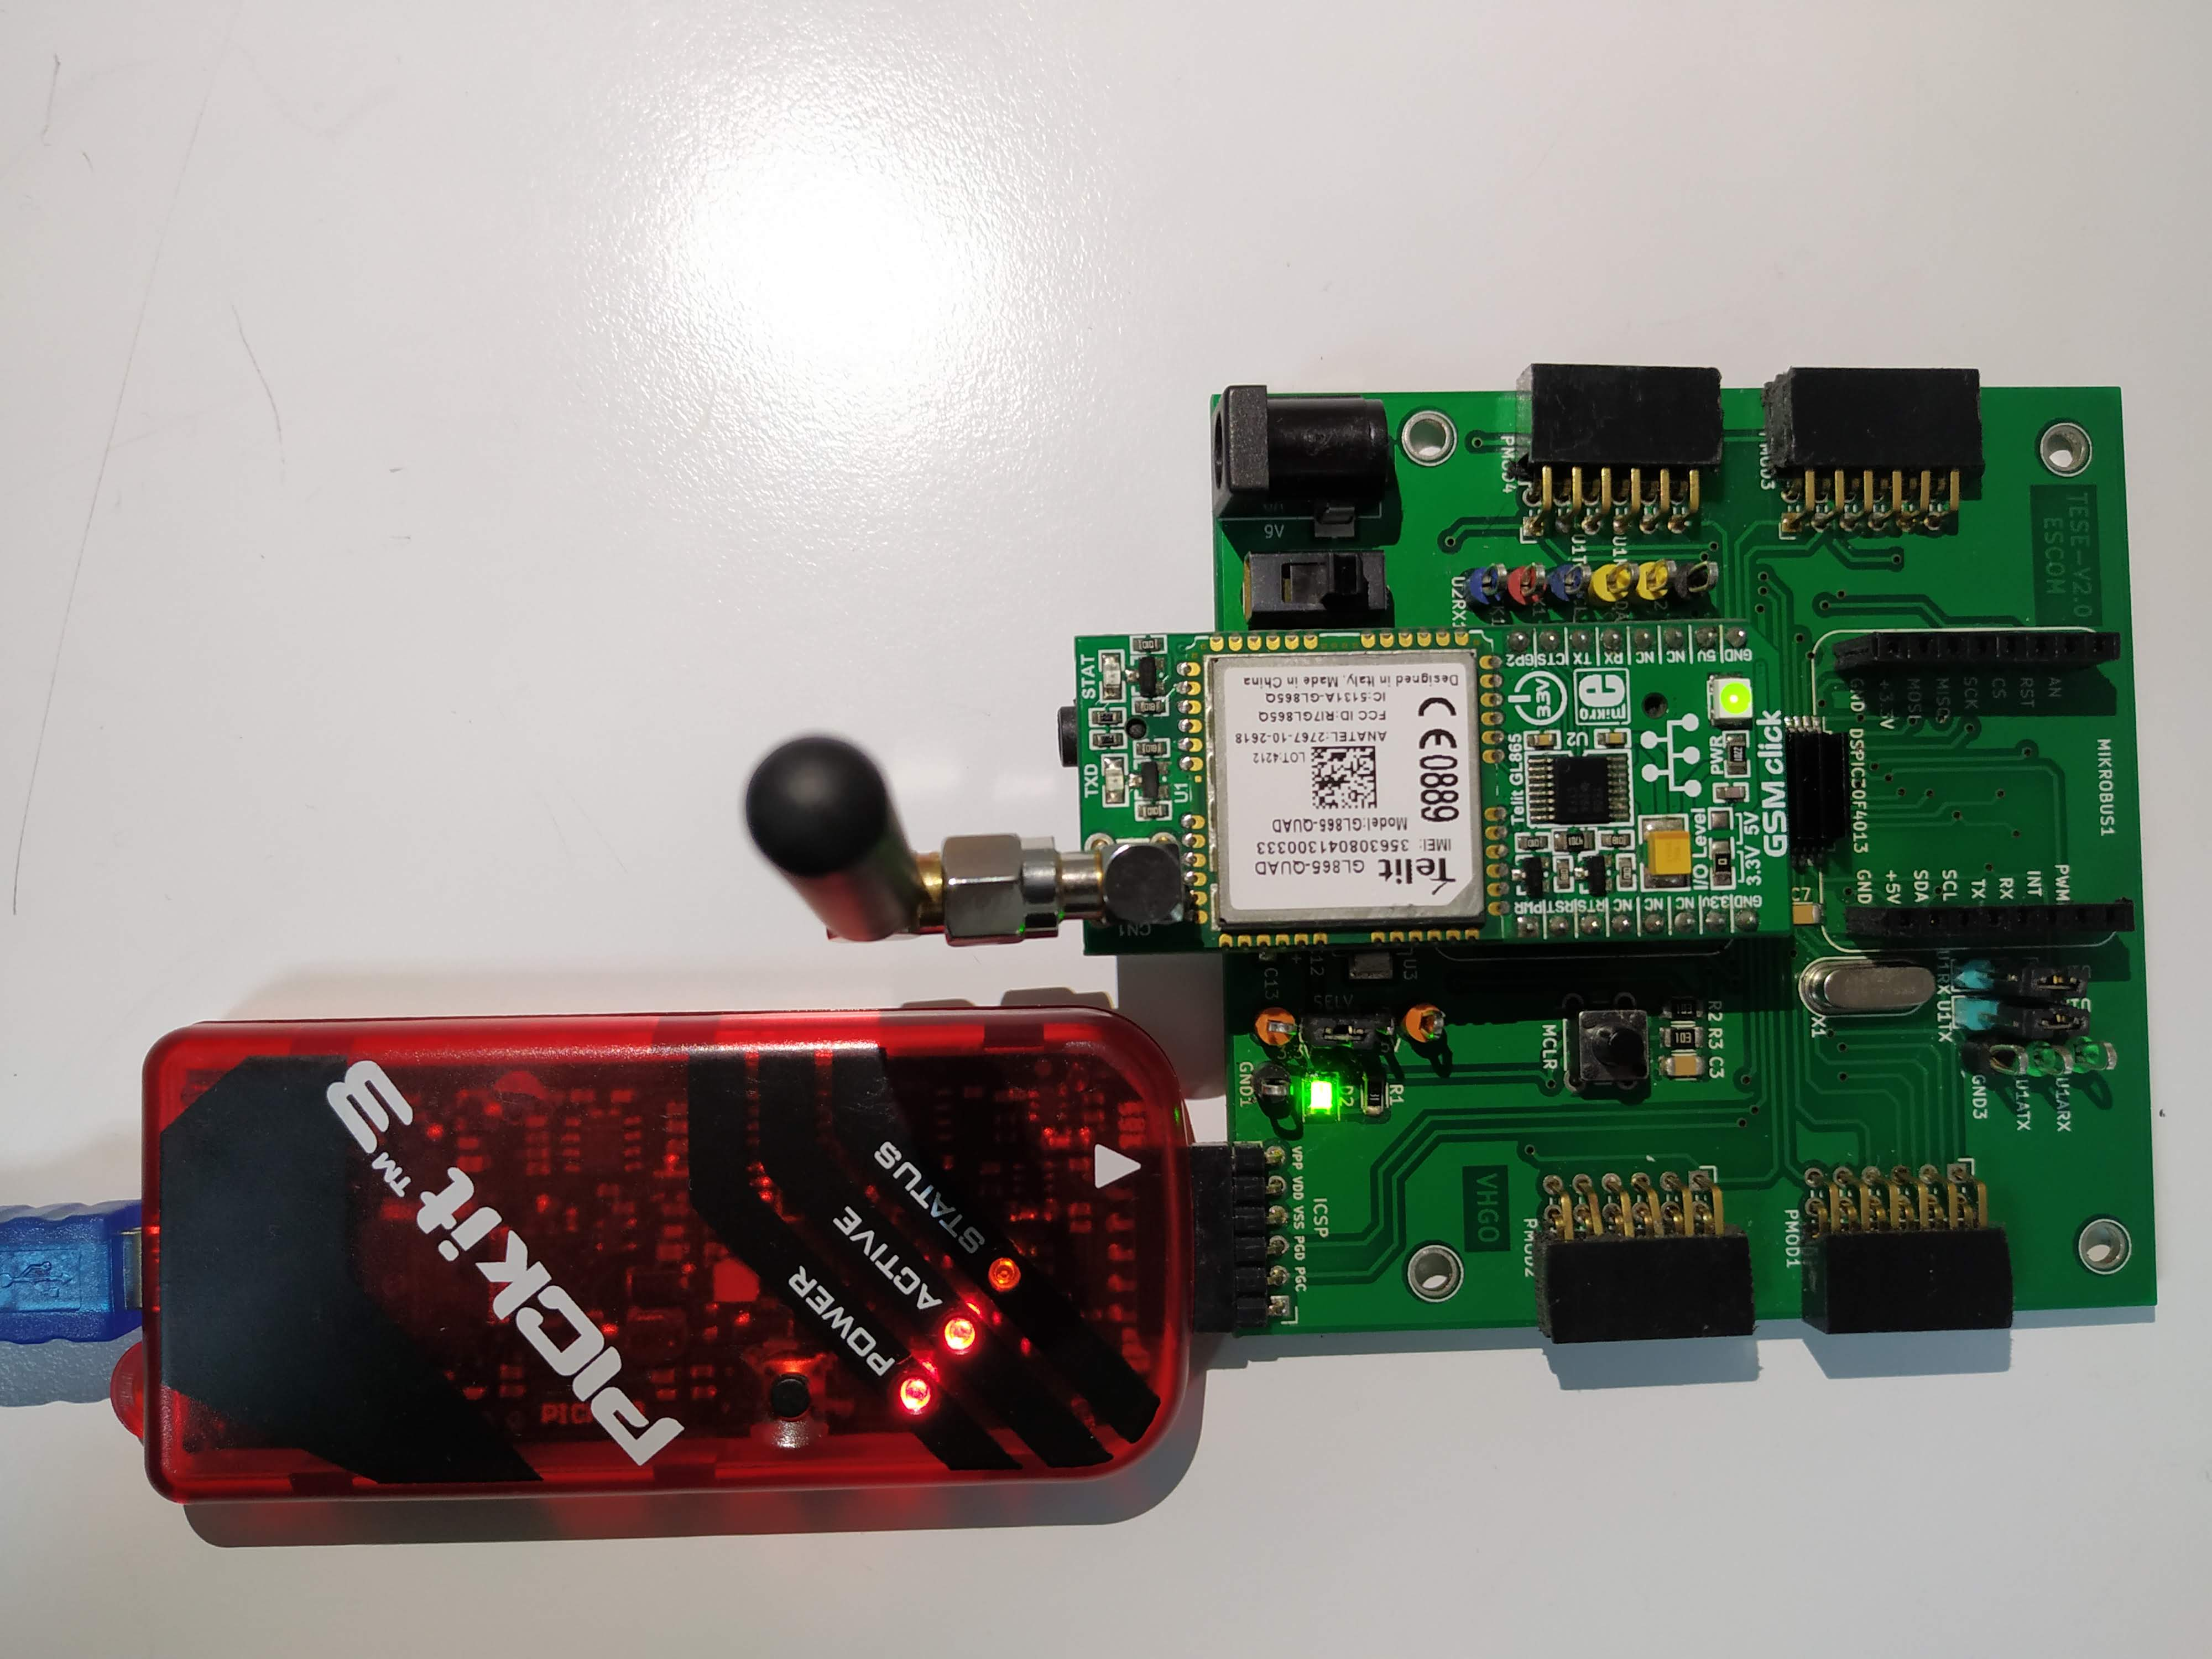
\includegraphics[width=2.5in]{AvancesPruebas/imagenes/ConexionFisicaGSM.jpg}
	\caption{Conexión del módulo 4G con el microcontrolador.}
	\label{fig:ConexionFisicaGSM}
\end{figure}


Para que se realice el envío del mensaje se consideraron las siguientes condiciones:
\begin{itemize}
	\item Que el resultado de frecuencia cardíaca se encuentre fuera del rango establecido ($50\ lpm$ - $100\ lpm$).
	\item Que el resultado de temperatura se encuentre fuera del rango establecido ($36^{\circ}C$ - $37^{\circ}C$).
	\item Que se agote un temporizador de minutos.
\end{itemize}

Si se cumple alguna de las condiciones anteriores, se obtiene la fecha y hora proporcionada por la red utilizada por el módulo de comunicación. Una vez que se tienen los tres datos (frecuencia cardíaca, temperatura y fecha y hora), se construye el mensaje de texto, cuyo cuerpo se definió de la siguiente manera: \textit{lpm:XX,temp:XX.XX,fecha:DD/MM/AAAA HH:MM}, y se realiza su envío. En la figura \ref{fig:RecepcionMsj} se muestra la captura de pantalla que contiene el mensaje recibido en el teléfono celular.

\begin{figure}[htbp!]
	\centering
	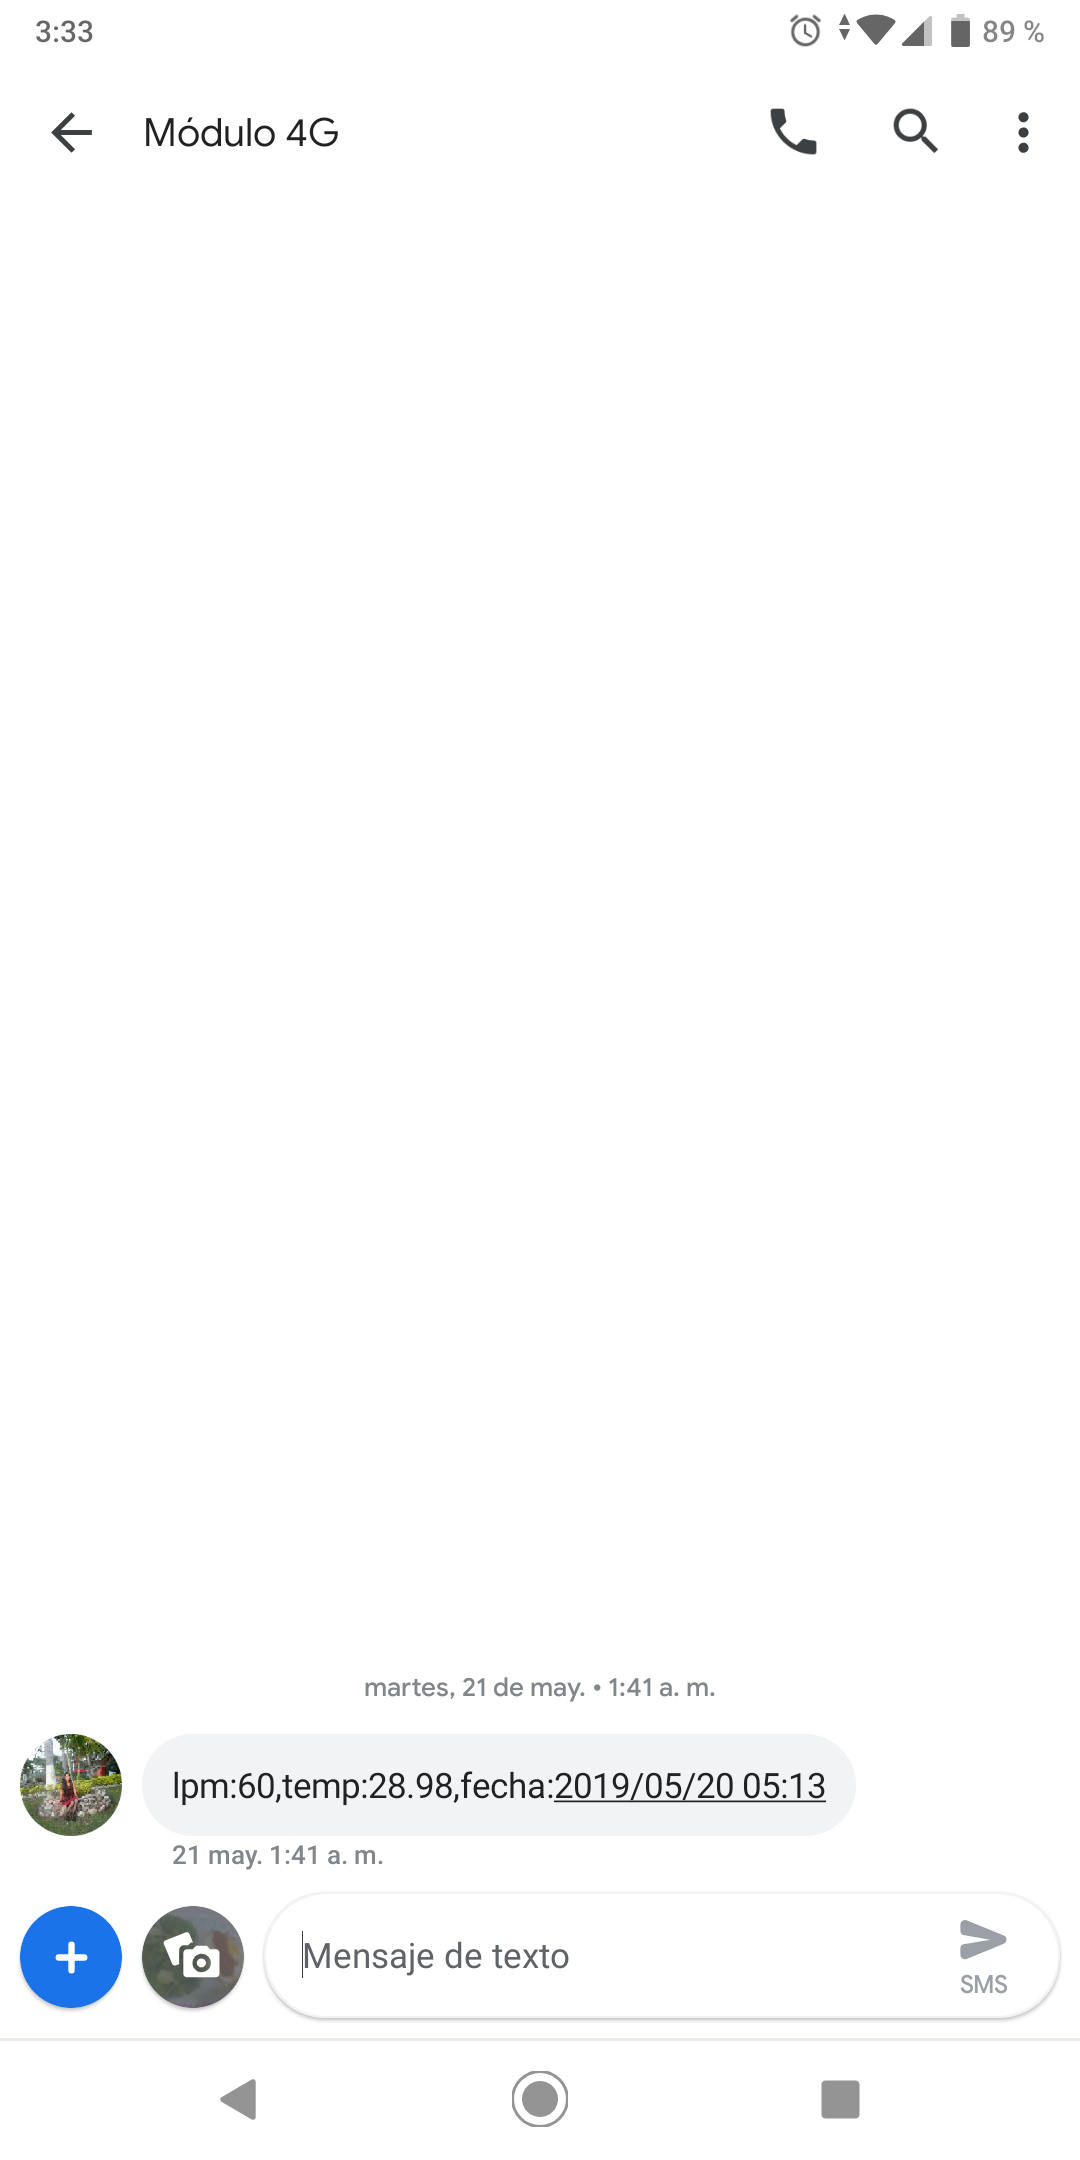
\includegraphics[width=2in]{AvancesPruebas/imagenes/formatoSMS.png}
	\caption{Recepción de mensaje enviado por el módulo 4G.}
	\label{fig:RecepcionMsj}
\end{figure}

\subsection{Aplicación móvil}
Se diseño una aplicación móvil en Android para ser utilizado en dispositivos con la versión 6.0 o posteriores. Esta aplicación permite al usuario registrar información de múltiples pacientes y consultar las mediciones de frecuencia cardíaca y temperatura corporal registradas de cada uno de ellos. Estas mediciones se obtienen automáticamente de los mensajes de texto recibidos en el teléfono móvil y son almacenadas en una base de datos. En la figura \ref{fig:casosUso:resumenUI5} se muestra una pantalla de la aplicación, en la que se muestran las mediciones registradas de un paciente.

\begin{figure}[htpb!]
	\begin{center}
		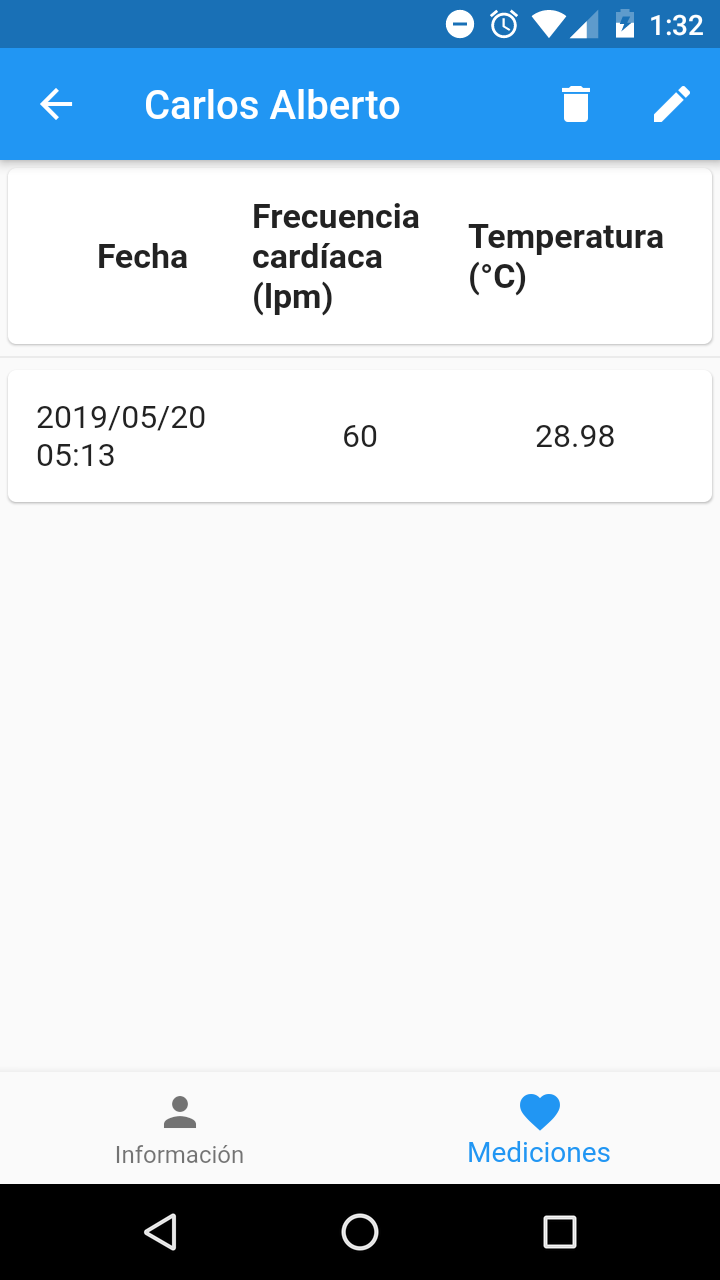
\includegraphics[width=2in]{AvancesPruebas/imagenes/app/ui_medicion.png}
		\caption{IU Consultar registros de signos vitales}
		\label{fig:casosUso:resumenUI5}
	\end{center}
\end{figure}

\section{Resultados}
Se logró realizar el diseño de un prototipo de sistema embebido que calcula la frecuencia cardíaca con una precisión del 98\%, que obtiene la temperatura corporal y realiza el envío de esta información en un mensaje de texto. \\

En la figura \ref{fig:integracion} se muestra la conexión del sensor de pulso, el sensor de temperatura y el módulo de comunicación con el microcontrolador, utilizando las conexiones proveídas por la tarjeta empleada durante este trabajo. \\

\begin{figure}[htbp!]
	\centering
	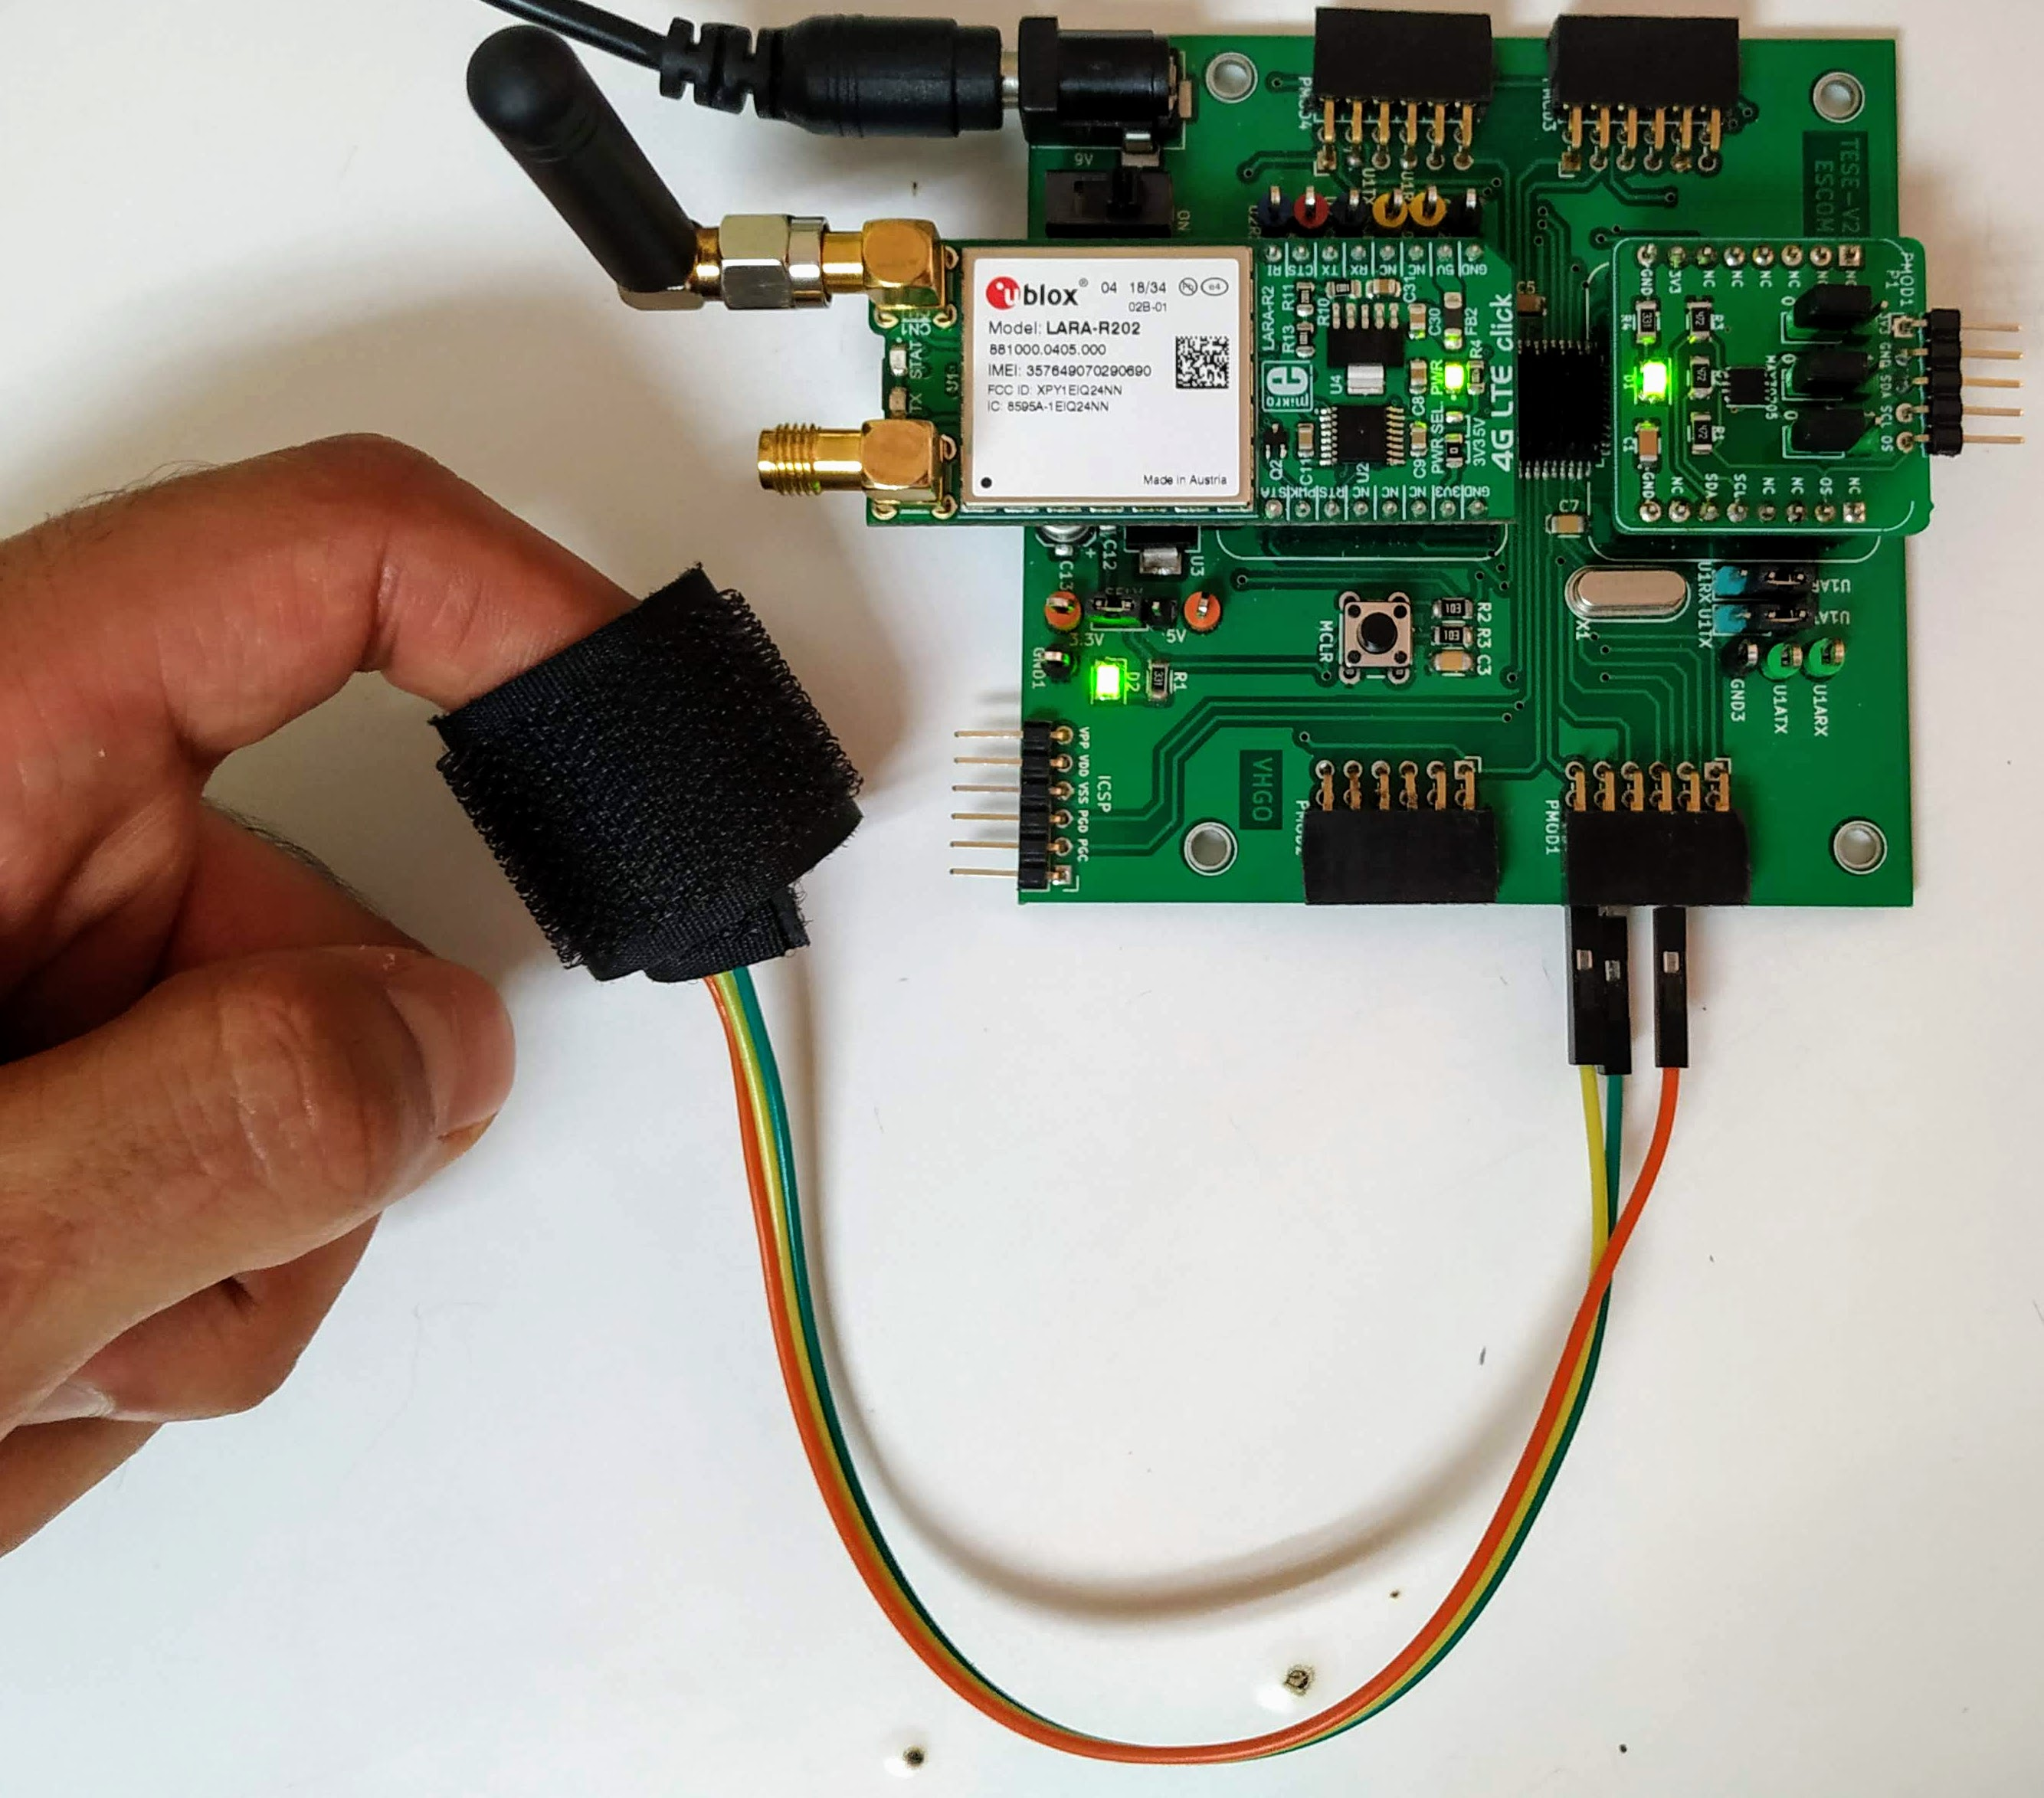
\includegraphics[width=2.5in]{AvancesPruebas/imagenes/integracion.jpg}
	\caption{Conexión del sistema embebido.}
	\label{fig:integracion}
\end{figure}

Se realizaron pruebas del sistema embebido obteniendo la frecuencia cardíaca 10 veces a 8 personas de diferentes edades, y comparando el resultado obtenido con el esperado obtenido con el método de palpación se calculó el error porcentual de los resultados de las pruebas. En las tablas \ref{table:resultado1} y \ref{table:resultado2} se muestran los resultados obtenidos del cálculo de la frecuencia cardíaca comparado con el valor esperado. \\

\begin{table}[htbp]
	\centering
	\subfloat[Resultados Persona 1][Resultados de la Persona 1 con 23 años de edad y frecuencia cardíaca de \textbf{75 lpm}]{
		\begin{tabular}{|l|l|}
			\hline
			\textbf{lpm obtenidos} & \textbf{Error (\%)} \\
			\hline \hline
			75 & 0 \\
			\hline
			73 & 2.67 \\
			\hline
			76 & 1.33 \\
			\hline
			74 & 1.33 \\
			\hline
			73 & 2.67 \\
			\hline
			73 & 2.67 \\
			\hline
			73 & 2.67 \\
			\hline
			76 & 1.33 \\
			\hline
			76 & 1.33 \\
			\hline
			77 & 2.67 \\
			\hline
		\end{tabular}}
	\qquad
	\subfloat[Resultados Persona 2][Resultados de la Persona 2 con 54 años de edad y frecuencia cardíaca de \textbf{57 lpm}]{
		\begin{tabular}{|l|l|}
			\hline
			\textbf{lpm obtenidos} & \textbf{Error (\%)} \\
			\hline \hline
			57 & 0 \\
			\hline
			55 & 3.51 \\
			\hline
			56 & 1.75 \\
			\hline
			56 & 1.75 \\
			\hline
			57 & 0 \\
			\hline
			58 & 1.75 \\
			\hline
			56 & 1.75 \\
			\hline
			57 & 0 \\
			\hline
			57 & 0 \\
			\hline
			57 & 0 \\
			\hline
		\end{tabular}}
	
	\subfloat[Resultados Persona 3][Resultados de la Persona 3 con 17 años de edad y frecuencia cardíaca de \textbf{80 lpm}]{
		\begin{tabular}{|l|l|}
			\hline
			\textbf{lpm obtenidos} & \textbf{Error (\%)} \\
			\hline \hline
			79 & 1.25 \\
			\hline
			80 & 0 \\
			\hline
			80 & 0 \\
			\hline
			82 & 2.5 \\
			\hline
			80 & 0 \\
			\hline
			81 & 1.25 \\
			\hline
			80 & 0 \\
			\hline
			79 & 1.25 \\
			\hline
			81 & 1.25 \\
			\hline
			80 & 0 \\
			\hline
		\end{tabular}}
	\qquad
	\subfloat[Resultados Persona 4][Resultados de la Persona 4 con 64 años de edad y frecuencia cardíaca de \textbf{64 lpm}]{
		\begin{tabular}{|l|l|}
			\hline
			\textbf{lpm obtenidos} & \textbf{Error (\%)} \\
			\hline \hline
			65 & 1.56 \\
			\hline
			65 & 1.56 \\
			\hline
			64 & 0 \\
			\hline
			66 & 3.13 \\
			\hline
			64 & 0 \\
			\hline
			64 & 0 \\
			\hline
			64 & 0 \\
			\hline
			67 & 4.69 \\
			\hline
			65 & 1.56 \\
			\hline
			64 & 0 \\
			\hline
		\end{tabular}}
	
	\caption{Resultados del cálculo de la frecuencia cardíaca de las Personas 1 a 4.}
	\label{table:resultado1}
\end{table}

\begin{table}[htbp]
	\centering
	\subfloat[Resultados Persona 5][Resultados de la Persona 5 con 7 años de edad y frecuencia cardíaca de \textbf{86 lpm}]{
		\begin{tabular}{|l|l|}
			\hline
			\textbf{lpm obtenidos} & \textbf{Error (\%)} \\
			\hline \hline
			85 & 1.16 \\
			\hline
			86 & 0 \\
			\hline
			85 & 1.16 \\
			\hline
			84 & 2.33 \\
			\hline
			87 & 1.16 \\
			\hline
			86 & 0 \\
			\hline
			86 & 0 \\
			\hline
			87 & 1.16 \\
			\hline
			85 & 1.16 \\
			\hline
			85 & 1.16 \\
			\hline
		\end{tabular}}
	\qquad
	\subfloat[Resultados Persona 6][Resultados de la Persona 6 con 46 años de edad y frecuencia cardíaca de \textbf{73 lpm}]{
		\begin{tabular}{|l|l|}
			\hline
			\textbf{lpm obtenidos} & \textbf{Error (\%)} \\
			\hline \hline
			70 & 4.11 \\
			\hline
			72 & 1.37 \\
			\hline
			73 & 0 \\
			\hline
			73 & 0 \\
			\hline
			73 & 0 \\
			\hline
			72 & 1.37 \\
			\hline
			74 & 1.37 \\
			\hline
			75 & 2.74 \\
			\hline
			72 & 1.37 \\
			\hline
			72 & 1.37 \\
			\hline
	\end{tabular}}
	
	\subfloat[Resultados Persona 7][Resultados de la Persona 7 con 15 años de edad y frecuencia cardíaca de \textbf{68 lpm}]{
		\begin{tabular}{|l|l|}
			\hline
			\textbf{lpm obtenidos} & \textbf{Error (\%)} \\
			\hline \hline
			67 & 1.47 \\
			\hline
			67 & 1.47 \\
			\hline
			68 & 0 \\
			\hline
			69 & 1.47 \\
			\hline
			68 & 0 \\
			\hline
			68 & 0 \\
			\hline
			67 & 1.47 \\
			\hline
			69 & 1.47 \\
			\hline
			69 & 1.47 \\
			\hline
			66 & 2.94 \\
			\hline
		\end{tabular}}
	\qquad
	\subfloat[Resultados Persona 8][Resultados de la Persona 8 con 35 años de edad y frecuencia cardíaca de \textbf{82 lpm}]{
		\begin{tabular}{|l|l|}
			\hline
			\textbf{lpm obtenidos} & \textbf{Error (\%)} \\
			\hline \hline
			80 & 2.44 \\
			\hline
			81 & 1.22 \\
			\hline
			81 & 1.22 \\
			\hline
			82 & 0 \\
			\hline
			82 & 0 \\
			\hline
			82 & 0 \\
			\hline
			83 & 1.22 \\
			\hline
			81 & 1.22 \\
			\hline
			82 & 0 \\
			\hline
			84 & 2.44 \\
			\hline
		\end{tabular}}
	
	\caption{Resultados del cálculo de la frecuencia cardíaca de las Personas 5 a 8.}
	\label{table:resultado2}
\end{table}

En la tabla \ref{sensorPulso:promedioError} se muestra el promedio de los errores obtenidos en las pruebas realizadas y se observa que se logró un error porcentual total de 1.17\%, que representa una diferencia de 1 o 2 latidos por minuto del resultado esperado.

\begin{table}[htbp]
	\begin{center}
		\begin{tabular}{|l|l|l|}
			\hline
			\textbf{Edad (años)} & \textbf{Frecuencia cardíaca (lpm)} & \textbf{Error (\%)} \\
			\hline \hline
			23 & 75 & 1.87 \\
			\hline
			54 & 60 & 1.05 \\
			\hline
			17 & 80 & 0.75 \\
			\hline
			15 & 68 & 1.18\\
			\hline
			7 & 86 & 0.93 \\
			\hline
			64 & 63 & 1.25 \\
			\hline
			46 & 73 & 1.37 \\
			\hline
			35 & 82 & 0.98 \\
			\hline
		\end{tabular}
		\caption{Promedio de error de las pruebas del cálculo de frecuencia cardíaca.}
		\label{sensorPulso:promedioError}
	\end{center}
\end{table}

Durante la ejecución de las pruebas se midió el tiempo en el que el sistema embebido realizaba las funciones programadas, siendo el menor tiempo posible para la recepción del mensaje de texto en el teléfono móvil de 27 segundos a partir del inicio de la toma de medición de los signos vitales de un paciente.


% An example of a floating figure using the graphicx package.
% Note that \label must occur AFTER (or within) \caption.
% For figures, \caption should occur after the \includegraphics.
% Note that IEEEtran v1.7 and later has special internal code that
% is designed to preserve the operation of \label within \caption
% even when the captionsoff option is in effect. However, because
% of issues like this, it may be the safest practice to put all your
% \label just after \caption rather than within \caption{}.
%
% Reminder: the "draftcls" or "draftclsnofoot", not "draft", class
% option should be used if it is desired that the figures are to be
% displayed while in draft mode.
%
%\begin{figure}[!t]
%\centering
%\includegraphics[width=2.5in]{myfigure}
% where an .eps filename suffix will be assumed under latex, 
% and a .pdf suffix will be assumed for pdflatex; or what has been declared
% via \DeclareGraphicsExtensions.
%\caption{Simulation results for the network.}
%\label{fig_sim}
%\end{figure}

% Note that the IEEE typically puts floats only at the top, even when this
% results in a large percentage of a column being occupied by floats.


% An example of a double column floating figure using two subfigures.
% (The subfig.sty package must be loaded for this to work.)
% The subfigure \label commands are set within each subfloat command,
% and the \label for the overall figure must come after \caption.
% \hfil is used as a separator to get equal spacing.
% Watch out that the combined width of all the subfigures on a 
% line do not exceed the text width or a line break will occur.
%
%\begin{figure*}[!t]
%\centering
%\subfloat[Case I]{\includegraphics[width=2.5in]{box}%
%\label{fig_first_case}}
%\hfil
%\subfloat[Case II]{\includegraphics[width=2.5in]{box}%
%\label{fig_second_case}}
%\caption{Simulation results for the network.}
%\label{fig_sim}
%\end{figure*}
%
% Note that often IEEE papers with subfigures do not employ subfigure
% captions (using the optional argument to \subfloat[]), but instead will
% reference/describe all of them (a), (b), etc., within the main caption.
% Be aware that for subfig.sty to generate the (a), (b), etc., subfigure
% labels, the optional argument to \subfloat must be present. If a
% subcaption is not desired, just leave its contents blank,
% e.g., \subfloat[].


% An example of a floating table. Note that, for IEEE style tables, the
% \caption command should come BEFORE the table and, given that table
% captions serve much like titles, are usually capitalized except for words
% such as a, an, and, as, at, but, by, for, in, nor, of, on, or, the, to
% and up, which are usually not capitalized unless they are the first or
% last word of the caption. Table text will default to \footnotesize as
% the IEEE normally uses this smaller font for tables.
% The \label must come after \caption as always.
%
%\begin{table}[!t]
%% increase table row spacing, adjust to taste
%\renewcommand{\arraystretch}{1.3}
% if using array.sty, it might be a good idea to tweak the value of
% \extrarowheight as needed to properly center the text within the cells
%\caption{An Example of a Table}
%\label{table_example}
%\centering
%% Some packages, such as MDW tools, offer better commands for making tables
%% than the plain LaTeX2e tabular which is used here.
%\begin{tabular}{|c||c|}
%\hline
%One & Two\\
%\hline
%Three & Four\\
%\hline
%\end{tabular}
%\end{table}


% Note that the IEEE does not put floats in the very first column
% - or typically anywhere on the first page for that matter. Also,
% in-text middle ("here") positioning is typically not used, but it
% is allowed and encouraged for Computer Society conferences (but
% not Computer Society journals). Most IEEE journals/conferences use
% top floats exclusively. 
% Note that, LaTeX2e, unlike IEEE journals/conferences, places
% footnotes above bottom floats. This can be corrected via the
% \fnbelowfloat command of the stfloats package.


\section{Conclusiones}
Con este proyecto terminal se realizó el diseño de un prototipo de sistema embebido para obtener la señal de pulso cardíaco  a partir de un sensor analógico de tipo fotopletismógrafo a la cual se le aplicaron técnicas de procesamiento digital de señales con la que se calculó la frecuencia cardíaca con una eficiencia de 98.83\% de acuerdo a las pruebas realizadas. Además se utilizó un sensor digital para la obtención de la temperatura y se realizó la configuración de un módulo de comunicación 3G/4G para el envío de la información obtenida mediante un mensaje de texto, que gracias a la implementación de una aplicación móvil le permitirá al usuario consultar las mediciones de diferentes pacientes.


% if have a single appendix:
%\appendix[Proof of the Zonklar Equations]
% or
%\appendix  % for no appendix heading
% do not use \section anymore after \appendix, only \section*
% is possibly needed

% use appendices with more than one appendix
% then use \section to start each appendix
% you must declare a \section before using any
% \subsection or using \label (\appendices by itself
% starts a section numbered zero.)
%

%
%\appendices
%\section{Proof of the First Zonklar Equation}
%Appendix one text goes here.
%
%% you can choose not to have a title for an appendix
%% if you want by leaving the argument blank
%\section{}
%Appendix two text goes here.


% use section* for acknowledgment
\section*{Reconocimientos}
Los Autores agradecen a la Escuela Superior de Cómputo
del Instituto Politécnico Nacional por el apoyo recibido y las
facilidades otorgadas para el desarrollo del presente trabajo
terminal. 


% Can use something like this to put references on a page
% by themselves when using endfloat and the captionsoff option.
\ifCLASSOPTIONcaptionsoff
  \newpage
\fi



% trigger a \newpage just before the given reference
% number - used to balance the columns on the last page
% adjust value as needed - may need to be readjusted if
% the document is modified later
%\IEEEtriggeratref{8}
% The "triggered" command can be changed if desired:
%\IEEEtriggercmd{\enlargethispage{-5in}}

% references section

% can use a bibliography generated by BibTeX as a .bbl file
% BibTeX documentation can be easily obtained at:
% http://mirror.ctan.org/biblio/bibtex/contrib/doc/
% The IEEEtran BibTeX style support page is at:
% http://www.michaelshell.org/tex/ieeetran/bibtex/
%\bibliographystyle{IEEEtran}
% argument is your BibTeX string definitions and bibliography database(s)
%\bibliography{IEEEabrv,../bib/paper}
%
% <OR> manually copy in the resultant .bbl file
% set second argument of \begin to the number of references
% (used to reserve space for the reference number labels box)
\begin{thebibliography}{1}

%\bibitem{IEEEhowto:kopka}
%H.~Kopka and P.~W. Daly, \emph{A Guide to \LaTeX}, 3rd~ed.\hskip 1em plus
%  0.5em minus 0.4em\relax Harlow, England: Addison-Wesley, 1999.

%%%%%Signos vitales
\bibitem{aguayoChile} Aguayo, A \& Lagos A (s.f.) Guía Clínica de Control de Signos Vitales. Universidad Pedro de Valdivia, Chile. Disponible en: \url{http://academico.upv.cl/doctos/KINE-4068/\%7B328B1B37-2C2A-4747-8B38-169806A27753%7D/2012/S1/GUIA%20TECNICA%20DE%20CONTROL%20DE%20SIGNOS%20VITALES%20KINE.pdf}
	
\bibitem{cobo2011} Cobo, D \& Daza, P (2011). Signos Vitales en Pediatría. Gastrohnup, 13(1), S58-S70. Disponible en: \url{http://bibliotecadigital.univalle.edu.co/bitstream/10893/5810/1/15%20signos.pdf} 

%\bibitem{signos2017} Signos Vitales (2017). Universidad Nacional de Mar del Plata, Argentina. 

\bibitem{valoresFreq} Frecuencia cardíaca normal en reposo. Disponible en: \url{https://www.medicalnewstoday.com/articles/291182.php}

\bibitem{signosvitales2016} Signos vitales (temperatura corporal, pulso, frecuencia respiratoria y presión arterial). (2016). University of Chicago Medicine. Disponible en: \url{http://healthlibrary.uchospitals.edu/Spanish/DiseasesConditions/Adult/NonTraumatic/85,P03963}
	
%%%%%Intro
\bibitem{ocde2016} OECD (2016), OECD Reviews of Health Systems: Mexico 2016, OECD Publishing, Paris. Disponible en: \url{http://dx.doi.org/10.1787/9789264230491-en}

%%%%Metodología
\bibitem{perez2006V} Perez, A.; et al. (2006). Una metodología para el desarrollo de hardware y software embebidos en sistemas críticos de seguridad. Systemics, Cybernetics and Informatics Journal, vol 3, Num. 2, pp. 70-75.

%%%%Embebidos
%\bibitem{vahid1999}	Vahid, F \& Givargis, F. (1999). Embedded System Design: An Unified Hardware/Software Approach. University of California Riverside. Disponible en: \url{https://pdfs.semanticscholar.org/3b62/7703e5b937954ec4637c04dc62637e218166.pdf}

%%%%%IoT
%\bibitem{vermesanIoT} Vermesan, O \& Friess, P. Internet of Things - From Research and Innovation to Market Deployment. Disponible en:  \url{http://www.internet-of-things-research.eu/pdf/IERC_Cluster_Book_2014_Ch.3_SRIA_WEB.pdf}
%
%\bibitem{laneIoT} N. D. Lane, E. Miluzzo, H. Lu, D. Peebles, T. Choudhury, and A. T.	Campbell, “A survey of mobile phone sensing,” IEEE Communications magazine, vol. 48, no. 9, 2010.
%
%\bibitem{arquitecturaIoT} Sikder, Amit Kumar \& Petracca, Giuseppe \& Aksu, Hidayet \& Jaeger, Trent \& Uluagac, Selcuk. (2018). A Survey on Sensor-based Threats to Internet-of-Things (IoT) Devices and Applications. 
	
\end{thebibliography}

% biography section
% 
% If you have an EPS/PDF photo (graphicx package needed) extra braces are
% needed around the contents of the optional argument to biography to prevent
% the LaTeX parser from getting confused when it sees the complicated
% \includegraphics command within an optional argument. (You could create
% your own custom macro containing the \includegraphics command to make things
% simpler here.)
%\begin{IEEEbiography}[{\includegraphics[width=1in,height=1.25in,clip,keepaspectratio]{mshell}}]{Michael Shell}
% or if you just want to reserve a space for a photo:

%\begin{IEEEbiography}{Michael Shell}
%Biography text here.
%\end{IEEEbiography}

% if you will not have a photo at all:
%\begin{IEEEbiographynophoto}{John Doe}
%Biography text here.
%\end{IEEEbiographynophoto}

% insert where needed to balance the two columns on the last page with
% biographies
%\newpage

%\begin{IEEEbiographynophoto}{Jane Doe}
%Biography text here.
%\end{IEEEbiographynophoto}

% You can push biographies down or up by placing
% a \vfill before or after them. The appropriate
% use of \vfill depends on what kind of text is
% on the last page and whether or not the columns
% are being equalized.

%\vfill

% Can be used to pull up biographies so that the bottom of the last one
% is flush with the other column.
%\enlargethispage{-5in}


% that's all folks
\end{document}
